%===============================================================================
% LaTeX sjabloon voor de bachelorproef toegepaste informatica aan HOGENT
% Meer info op https://github.com/HoGentTIN/latex-hogent-report
%===============================================================================

\documentclass[dutch,dit,thesis]{hogentreport}

% TODO:
% - If necessary, replace the option `dit`' with your own department!
%   Valid entries are dbo, dbt, dgz, dit, dlo, dog, dsa, soa
% - If you write your thesis in English (remark: only possible after getting
%   explicit approval!), remove the option "dutch," or replace with "english".

\usepackage{listings}
\usepackage{glossaries}

%% Pictures to include in the text can be put in the graphics/ folder
\graphicspath{{../graphics/}}

%% For source code highlighting, requires pygments to be installed
%% Compile with the -shell-escape flag!
\usepackage[section]{minted}
%% If you compile with the make_thesis.{bat,sh} script, use the following
%% import instead:
%% \usepackage[section,outputdir=../output]{minted}
\usemintedstyle{solarized-light}
\definecolor{bg}{RGB}{253,246,227} %% Set the background color of the codeframe

%% Change this line to edit the line numbering style:
\renewcommand{\theFancyVerbLine}{\ttfamily\scriptsize\arabic{FancyVerbLine}}

%% Macro definition to load external java source files with \javacode{filename}:
\newmintedfile[javacode]{java}{
    bgcolor=bg,
    fontfamily=tt,
    linenos=true,
    numberblanklines=true,
    numbersep=5pt,
    gobble=0,
    framesep=2mm,
    funcnamehighlighting=true,
    tabsize=4,
    obeytabs=false,
    breaklines=true,
    mathescape=false
    samepage=false,
    showspaces=false,
    showtabs =false,
    texcl=false,
}

% Other packages not already included can be imported here

%%---------- Document metadata -------------------------------------------------
% TODO: Replace this with your own information
\author{Lander De Kesel}
\supervisor{Dhr. Gertjan Bosteels}
\cosupervisor{Dhr. Kris Van Opstaele}
\title%
    {Authenticatie en Autorisatie in applicatieontwikkeling, hoe kan dit makkelijk worden aangeboden: Een diepgaande analyse en implementatie.}
\academicyear{\advance\year by -1 \the\year--\advance\year by 1 \the\year}
\examperiod{1}
\degreesought{\IfLanguageName{dutch}{Professionele bachelor in de toegepaste informatica}{Bachelor of applied computer science}}
\partialthesis{false} %% To display 'in partial fulfilment'
%\institution{Internshipcompany BVBA.}

%% Add global exceptions to the hyphenation here
\hyphenation{back-slash}

%% The bibliography (style and settings are  found in hogentthesis.cls)
\addbibresource{bachproef.bib}            %% Bibliography file
\addbibresource{../voorstel/voorstel.bib} %% Bibliography research proposal
\defbibheading{bibempty}{}

%% Prevent empty pages for right-handed chapter starts in twoside mode
\renewcommand{\cleardoublepage}{\clearpage}

\renewcommand{\arraystretch}{1.2}

\makeglossaries
\newacronym{sso}{SSO}{Single Sign On}
\newacronym{jwt}{JWT}{JSON Web Token}
\newacronym{jwts}{JWTs}{JSON Web Tokens}
\newacronym{jwe}{JWE}{JSON Web Encryption}
\newacronym{jws}{JWS}{JSON Web Signature}
\newacronym{idaas}{IDaaS}{Identity as a Service}
\newacronym{iam}{IAM}{Identity and Access Management}
\newacronym{mfa}{MFA}{Multi-Factor Authentication}
\newacronym{api}{API}{Application Programming Interface}
\newacronym{aws}{AWS}{Amazon Web Services}
\newacronym{iap}{IAP}{Identity and Access Proxy}
\newacronym{cas}{CAS}{Central Authentication Service}
\newacronym{oidc}{OIDC}{OpenID Connect}
\newacronym{ldap}{LDAP}{Lightweight Directory Access Protocol}
\newacronym{otp}{OTP}{One-Time Passwords}
\newacronym{sdk}{SDK}{Software Development Kit}
\newacronym{auth}{Auth}{Authenticatie en Autorisatie}
\newacronym{csrf}{CSRF}{Cross-Site Request Forgery}
\newacronym{http}{HTTP}{Hypertext Transfer Protocol}
\newacronym{tls}{TLS}{Transport Layer Security}
\newacronym{json}{JSON}{JavaScript Object Notation}
\newacronym{w3c}{W3C}{World Wide Web Consortium}

%% Content starts here.
\begin{document}

%---------- Front matter -------------------------------------------------------

\frontmatter

\hypersetup{pageanchor=false} %% Disable page numbering references
%% Render a Dutch outer title page if the main language is English
\IfLanguageName{english}{%
    %% If necessary, information can be changed here
    \degreesought{Professionele Bachelor toegepaste informatica}%
    \begin{otherlanguage}{dutch}%
       \maketitle%
    \end{otherlanguage}%
}{}

%% Generates title page content
\maketitle
\hypersetup{pageanchor=true}

%%=============================================================================
%% Voorwoord
%%=============================================================================

\chapter*{\IfLanguageName{dutch}{Woord vooraf}{Preface}}%
\label{ch:voorwoord}

%% TODO:
%% Het voorwoord is het enige deel van de bachelorproef waar je vanuit je
%% eigen standpunt (``ik-vorm'') mag schrijven. Je kan hier bv. motiveren
%% waarom jij het onderwerp wil bespreken.
%% Vergeet ook niet te bedanken wie je geholpen/gesteund/... heeft

Het schrijven van deze bachelorproef was een uitdagende en heel verrijkende ervaring. Het onderwerp ``authenticatie en autorisatie in applicatie ontwikkeling'' heeft altijd mijn interesse gewekt, 
vooral vanwege de cruciale rol die authenticatie en autorisatie speelt in de huidige digitale wereld. Het was een kans om dit onderwerp grondiger te onderzoeken en de complexiteit ervan te begrijpen.
Ik heb dit onderzoek gekozen omdat ik al sinds het begin van mijn opleiding, en zelfs daarvoor, geïnteresseerd ben in beveiliging en privacy bescherming. Het is een onderwerp dat steeds belangrijker wordt 
in de digitale wereld, en ik wilde graag meer leren over de verschillende aspecten ervan. Dit onderzoek heeft me geholpen om een beter inzicht te krijgen in de uitdagingen en oplossingen op het gebied van
authenticatie en autorisatie in applicatie ontwikkeling.
\newline
Ik ben al altijd bezig geweest met het beveiligen, of ten minste poging tot beveiligen, van mijn eigen applicaties en websites. Vaak gebruikte ik bestaande oplossingen/aanbieders, maar ik heb altijd al ``meer'' gewild.
Ik wilde meer weten over hoe deze systemen werken, meer weten over hoe ik dit ooit zelf zou kunnen implementeren. Daarom ben ik, een jaar voor dit onderzoek, begonnen met informatie te verzamelen en
het effectief ontwikkelen van een eigen authenticatie- en autorisatie systeem. Maar ik wist dat ik iets miste, ik wist dat er nog veel meer te leren was.
\newline
Daarom ben ik begonnen met dit onderzoek. Ik zag dit als de ultieme kans om meer te leren over dit onderwerp, en om mijn kennis te delen met anderen.
Ik ben vrij zeker dat ik nu zo goed als alle kennis en informatie heb verzameld die ik nodig heb om een veilig en betrouwbaar authenticatie- en autorisatie systeem te ontwikkelen. Ook hoop ik dat dit
onderzoek anderen kan helpen met hetzelfde doel, of toch ten minste een beter begrip kan geven van de complexiteit van dit onderwerp.
\newline
\newline
Ik wil graag mijn promotor, de heer Gertjan Bosteels, en mijn co-promotor, de heer Kris Van Opstaele, bedanken voor hun waardevolle feedback en begeleiding gedurende dit proces. Hun inzichten en suggesties hebben enorm bijgedragen aan de kwaliteit van dit werk. 
\newline
\newline
Ik hoop dat dit werk nuttig zal zijn voor andere ontwikkelaars die geconfronteerd worden met de uitdagingen van authenticatie en autorisatie in applicatie ontwikkeling.

\begin{flushright}
Lander De Kesel
\end{flushright}
%%=============================================================================
%% Samenvatting
%%=============================================================================

% TODO: De "abstract" of samenvatting is een kernachtige (~ 1 blz. voor een
% thesis) synthese van het document.
%
% Een goede abstract biedt een kernachtig antwoord op volgende vragen:
%
% 1. Waarover gaat de bachelorproef?
% 2. Waarom heb je er over geschreven?
% 3. Hoe heb je het onderzoek uitgevoerd?
% 4. Wat waren de resultaten? Wat blijkt uit je onderzoek?
% 5. Wat betekenen je resultaten? Wat is de relevantie voor het werkveld?
%
% Daarom bestaat een abstract uit volgende componenten:
%
% - inleiding + kaderen thema
% - probleemstelling
% - (centrale) onderzoeksvraag
% - onderzoeksdoelstelling
% - methodologie
% - resultaten (beperk tot de belangrijkste, relevant voor de onderzoeksvraag)
% - conclusies, aanbevelingen, beperkingen
%
% LET OP! Een samenvatting is GEEN voorwoord!

%%---------- Nederlandse samenvatting -----------------------------------------
%
% TODO: Als je je bachelorproef in het Engels schrijft, moet je eerst een
% Nederlandse samenvatting invoegen. Haal daarvoor onderstaande code uit
% commentaar.
% Wie zijn bachelorproef in het Nederlands schrijft, kan dit negeren, de inhoud
% wordt niet in het document ingevoegd.

\IfLanguageName{english}{%
\selectlanguage{dutch}
\chapter*{Samenvatting}
\lipsum[1-4]
\selectlanguage{english}
}{}

%%---------- Samenvatting -----------------------------------------------------
% De samenvatting in de hoofdtaal van het document

\chapter*{\IfLanguageName{dutch}{Samenvatting}{Abstract}}

Dit onderzoeksvoorstel richt zich op de specifieke uitdagingen met betrekking tot authenticatie en autorisatie in applicatieontwikkeling, met als primaire 
focus het vereenvoudigen van deze processen. Het doel is om praktische oplossingen te identificeren die relevant zijn voor ontwikkelaars 
die in hun projecten worden geconfronteerd met problemen op het gebied van beveiliging en gebruikerservaring. Dit aan de hand van een diepgaande analyse,
onderzoek en vergelijking van bestaande oplossingen/providers en technologieën/methoden, om zo de meest geschikte en effectieve aanpak te bepalen. 
\newline
\newline
Het onderzoek wordt aangedreven door de aanvankelijke uitdagingen bij het beveiligen en toegankelijk maken van applicaties, met authenticatie en 
autorisatie als cruciale aspecten. Het richt zich op het bieden van een oplossing voor het beveiligen van diverse soorten apps, zoals desktop-, 
web- en mobiele apps. Vandaag de dag zijn er al heel wat opties aanwezig hoe men authenticatie en autorisatie kan implementeren in hun applicaties.
Het doel is dus om te achterhalen hoe dit kan worden aangeboden aan elke ontwikkelaar.
\newline
\newline
Er zal een grondige analyse worden uitgevoerd van bestaande oplossingen en technologieën. Als eerst worden de bestaande technologieën onderzocht,
dit om een grondige kennis te verkrijgen over hoe deze functioneren en vooral hoe deze kunnen worden geïmplementeerd indien men kies een eigen
authenticatieserver te ontwikkelen. Vervolgens zullen bestaande oplossingen worden geanalyseerd om inzicht te krijgen wat de standaarden zijn die
men gebruikt bij de ontwikkeling van een authenticatieserver. 
Door het opstellen van de vergelijkingscriteria, kan er een duidelijk beeld worden geschetst van de voor- en nadelen van elke provider.
Maar vooral om te kijken of men al dan niet kan vaststellen dat dit hun antwoord is.
Indien men niet wil afhangen van een derde partij gaan we verder: de analyse of een lichtgewicht instantie, die bijvoorbeeld op een Docker image
kan draaien, bestaat of niet. Indien dit nog niet bestaat zal er een proof-of-concept worden ontwikkeld, de Docker image zal OAuth 2.0
autorisatie framework gaan ontwikkelen. Indien dit wel al bestaat zal een vergelijkende studie bestaande alternatieven vergelijken en suggereren.
\newline
\newline
Uit het onderzoek word er veel kennis opgedaan omtrent de bestaande auth technologieën. Met de informatie die beschikbaar is door deze analyse
zou een ontwikkelaar een eigen authenticatieserver kunnen ontwikkelen. Vervolgens concluderen we uit het huidig onderzoekt dat er al veel bestaande 
providers zijn, maar dat deze vaak beperkingen opleggen en kosten met zich meebrengen. Als men graag zelf iets implementeert, maar niet volledig
van nul wilt beginnen, kan men er voor kiezen een lichtgewicht instantie te ontwikkelen. Door dit domein verder te onderzoeken, werd vastgesteld 
dat deze reeds bestonden. Daarom werd er vervolgens voor gekozen om een vergelijkende studie te houden over de bestaande alternatieven. Uit deze
studie bleek het al snel dat er maar drie overbleven: Keycloak, Hydra en Oathkeeper. Het resultaat van dit onderzoek stelt dus vast dat men een bestaande
lichtgewicht instantie kan implementeren, zoals Keycloak, als men volledige controle wil. Het tweede alternatief is een bestaande oplossing/provider
gebruiken, houd er wel rekening mee dat dit beperkingen en kosten kan met zich meebrengen. Het derde en laatste alternatief, dat vaak het minst zal
gekozen worden, is om zelf een authenticatieserver te ontwikkelen die bijvoorbeeld het OAuth 2.0 autorisatie framework implementeert. Dit laatste alternatief
zal de meeste inspanning kosten, maar zal ongetwijfeld de meeste kennis en ervaring opleveren.
\newline
\newline
Conclusie: authenticatie en autorisatie in applicatieontwikkeling is al veel verder ontwikkeld dan initiëel gedacht bij het begin van dit onderzoek.
Dit onderzoek werd gestart met weinig kennis over auth en werd beëindigd met een grondige basis om zelf een authenticatieserver te ontwikkelen.
Maar dit is niet de echte conclusie van dit onderzoek. Als een ontwikkelaar of een bedrijf authenticatie en autorisatie in hun applicaties wil
integreren, kunnen we concluderen dat er vaak zal gegrepen worden naar een bestaande provider. Dit is de makkelijkste weg, maar vaak niet de
goedkoopste weg. Vaak denken bedrijven alleen aan de korte termijn voordelen en zal er vaak op lange termijn worden ingezien dat er een andere
mogelijkheid was. Zoals een Docker image van Keycloak bijvoorbeeld, die on-premise draait. Of men kan nog verder gaan: een zelf ontwikkelde
authenticatieserver implementeren die het OAuth 2.0 autorisatie framework implementeert. Wat gesuggereerd wordt: bij weinig ervaring gebruikt men
best een bestaande provider, bij matige ervaring kan men Keycloak on-premise gebruiken, en als laatste bij voldoende ervaring kan men een zelf
ontwikkelde authenticatieserver implementeren die het OAuth 2.0 autorisatie framework implementeert.


%---------- Inhoud, lijst figuren, ... -----------------------------------------

\tableofcontents

% In a list of figures, the complete caption will be included. To prevent this,
% ALWAYS add a short description in the caption!
%
%  \caption[short description]{elaborate description}
%
% If you do, only the short description will be used in the list of figures

\listoffigures

% If you included tables and/or source code listings, uncomment the appropriate
% lines.
\listoftables
\listoflistings

% Als je een lijst van afkortingen of termen wil toevoegen, dan hoort die
% hier thuis. Gebruik bijvoorbeeld de ``glossaries'' package.
% https://www.overleaf.com/learn/latex/Glossaries
\printglossaries

%---------- Kern ---------------------------------------------------------------

\mainmatter{}

% De eerste hoofdstukken van een bachelorproef zijn meestal een inleiding op
% het onderwerp, literatuurstudie en verantwoording methodologie.
% Aarzel niet om een meer beschrijvende titel aan deze hoofdstukken te geven of
% om bijvoorbeeld de inleiding en/of stand van zaken over meerdere hoofdstukken
% te verspreiden!

%%=============================================================================
%% Inleiding
%%=============================================================================

\chapter{\IfLanguageName{dutch}{Inleiding}{Introduction}}%
\label{ch:inleiding}

In de hedendaagse digitale wereld zijn applicaties niet meer weg te denken uit ons dagelijks leven. Of het nu gaat om desktop-, web- of mobiele applicaties, ze vormen de ruggengraat van moderne interactie 
en dienstverlening. Echter, met de toename van digitale transacties en gegevensuitwisseling, worden veiligheidsaspecten zoals authenticatie en autorisatie steeds belangrijker. Het beveiligen van deze applicaties 
terwijl een naadloze gebruikerservaring behouden blijft, vormt een uitdagende taak voor ontwikkelaars.
\newline
\newline
Dit onderzoeksvoorstel richt zich op de specifieke uitdagingen met betrekking tot authenticatie en autorisatie in applicatieontwikkeling. Het beoogt deze processen te vereenvoudigen en praktische oplossingen 
te identificeren en implementeren die relevant zijn voor ontwikkelaars die met beveiliging- en gebruikerservaring problemen worden geconfronteerd. Hierbij wordt een diepgaande analyse, onderzoek en 
vergelijking van bestaande oplossingen en technologieën uitgevoerd om de meest geschikte en effectieve aanpak te bepalen.
\newline
\newline
Het onderzoek wordt gestimuleerd door de initiële uitdagingen bij het beveiligen en toegankelijk maken van applicaties, waarbij authenticatie en autorisatie als cruciale aspecten worden beschouwd. 
Er wordt gestreefd naar het bieden van een referentie-implementatie die ontwikkelaars kunnen gebruiken om hun eigen applicaties te beveiligen, zonder afhankelijk te zijn van externe diensten of aanbieders die vaak beperkingen opleggen en kosten met zich meebrengen.
\newline
\newline
Door middel van een iteratieve aanpak zal dit onderzoek zich richten op het identificeren van de belangrijkste uitdagingen en het ontwikkelen van oplossingen die deze uitdagingen aanpakken. 
Hierbij zal een grondige analyse worden uitgevoerd van bestaande oplossingen en technologieën, waarbij de nadruk ligt op het bieden van een eenvoudige, effectieve en veilige oplossing.
\newline
\newline
Het doel van dit onderzoek is om ontwikkelaars die specifieke uitdagingen ervaren bij het implementeren van effectieve authenticatie- en autorisatiesystemen, te ondersteunen en richtlijnen te bieden om deze uitdagingen te overwinnen.
De focus ligt op concrete problemen waarmee ontwikkelaars worden geconfronteerd, zoals beveiligingslekken, complexe implementaties en gebruikerservaring problemen.


\section{\IfLanguageName{dutch}{Probleemstelling}{Problem Statement}}%
\label{sec:probleemstelling}
In de huidige digitale wereld is de beveiliging van applicaties een cruciaal aspect geworden. Authenticatie en autorisatie zijn twee belangrijke veiligheidsaspecten die een uitdaging vormen voor ontwikkelaars. 
Het implementeren van deze aspecten op een manier die zowel veilig als gebruiksvriendelijk is, is vaak complex en tijdrovend. Bovendien kunnen fouten in de implementatie leiden tot ernstige beveiligingslekken. 
\newline
Daarnaast zijn veel bestaande oplossingen afhankelijk van externe diensten of aanbieders, die vaak beperkingen opleggen en kosten met zich meebrengen. Dit kan een belemmering vormen voor ontwikkelaars, 
vooral voor diegenen die werken aan kleinere projecten of met beperkte budgetten.
\newline
Het doel van dit onderzoek is om bestaande oplossingen en technologieën voor authenticatie en autorisatie in applicatieontwikkeling te analyseren, vergelijken en evalueren. 
Het onderzoek richt zich op het identificeren van pijnpunten en het doen van suggesties om ontwikkelaars een duidelijke richtlijn te bieden voor het implementeren van veilige applicaties. 
Het doel is om ontwikkelaars te ondersteunen bij het overwinnen van uitdagingen op het gebied van beveiliging en gebruikerservaring.

\section{\IfLanguageName{dutch}{Onderzoeksvraag}{Research question}}%
\label{sec:onderzoeksvraag}

De centrale onderzoeksvraag van dit onderzoek is: ``Hoe kunnen ontwikkelaars effectieve en veilige authenticatie- en autorisatiesystemen implementeren in applicaties, zonder afhankelijk te zijn van 
externe diensten of aanbieders, en tegelijkertijd een optimale gebruikerservaring bieden?''
\newline
\newline
Deze centrale onderzoeksvraag kan verder worden opgesplitst in de volgende deelvragen:
\newline
\newline
1. Wat zijn de huidige uitdagingen en problemen bij het implementeren van authenticatie en autorisatie in applicaties?
\newline
2. Welke bestaande oplossingen en technologieën zijn er momenteel beschikbaar voor het implementeren van authenticatie en autorisatie in applicaties, en wat zijn hun voor- en nadelen?
\newline
3. Hoe kunnen deze oplossingen en technologieën worden verbeterd of aangepast om de uitdagingen en problemen aan te pakken die ontwikkelaars tegenkomen?


\section{\IfLanguageName{dutch}{Onderzoeksdoelstelling}{Research objective}}%
\label{sec:onderzoeksdoelstelling}

Het beoogde resultaat van dit onderzoek is een grondige analyse van bestaande oplossingen en technologieën voor authenticatie en autorisatie in applicatieontwikkeling, en het voorstellen van 
verbeteringen of aanpassingen om de uitdagingen en problemen die ontwikkelaars tegenkomen aan te pakken. 
\newline
\newline
Het succes van dit onderzoek zal worden gemeten aan de hand van de volgende criteria:
\newline
\newline
1. Het identificeren van de belangrijkste uitdagingen en problemen bij het implementeren van authenticatie en autorisatie in applicaties.
\newline
2. Het uitvoeren van een grondige analyse van bestaande oplossingen en technologieën, en het identificeren van hun voor- en nadelen.
\newline
3. Het voorstellen van verbeteringen of aanpassingen aan deze oplossingen en technologieën om de geïdentificeerde uitdagingen en problemen aan te pakken.
\newline
4. Het opstellen van een verslag met aanbevelingen op basis van een vergelijkende studie van de geanalyseerde oplossingen en technologieën.
\newline
\newline
Het uiteindelijke doel is om ontwikkelaars te ondersteunen bij het overwinnen van uitdagingen op het gebied van beveiliging en gebruikerservaring, en hen te helpen bij het bouwen van veilige en 
gebruiksvriendelijke applicaties.

\section{\IfLanguageName{dutch}{Opzet van deze bachelorproef}{Structure of this bachelor thesis}}%
\label{sec:opzet-bachelorproef}

% Het is gebruikelijk aan het einde van de inleiding een overzicht te
% geven van de opbouw van de rest van de tekst. Deze sectie bevat al een aanzet
% die je kan aanvullen/aanpassen in functie van je eigen tekst.

Deze bachelorproef is als volgt opgebouwd:

In Hoofdstuk~\ref{ch:stand-van-zaken} wordt een overzicht gegeven van de stand van zaken binnen het onderzoeksdomein, op basis van een literatuurstudie.

In Hoofdstuk~\ref{ch:methodologie} wordt de methodologie toegelicht en worden de gebruikte onderzoekstechnieken besproken om een antwoord te kunnen formuleren op de onderzoeksvragen.

% TODO: Vul hier aan voor je eigen hoofdstukken, één of twee zinnen per hoofdstuk

In Hoofdstuk~\ref{ch:conclusie}, tenslotte, wordt de conclusie gegeven en een antwoord geformuleerd op de onderzoeksvragen. Daarbij wordt ook een aanzet gegeven voor toekomstig onderzoek binnen dit domein.
\chapter{\IfLanguageName{dutch}{Stand van zaken}{State of the art}}%
\label{ch:stand-van-zaken}

% Tip: Begin elk hoofdstuk met een paragraaf inleiding die beschrijft hoe
% dit hoofdstuk past binnen het geheel van de bachelorproef. Geef in het
% bijzonder aan wat de link is met het vorige en volgende hoofdstuk.

% Pas na deze inleidende paragraaf komt de eerste sectiehoofding.

\section{Auth technologieën}%
\label{sec:auth-technologieën}
In eerste instantie wordt bekeken welke huidge technologieën er vandaag de dag bestaan en welke de meest gebruikte zijn. Dit omdat er eerst een goede kennis
moet worden gelegd van de huidige technologieën vooraleer er kan worden overgegaan naar de volgende stappen.


\subsection{OAuth 2.0}%
\label{subsec:oauth-2.0}
\autocite{Hardt2012}
OAuth 2.0 wordt gebruikt om toegang tot bronnen te delegeren zonder gebruikersreferenties te delen. Het is een autorisatie framework en wordt dus niet gebruikt voor het authenticeren van gebruikers. Vaak gebruikt om Single Sign On (SSO) en toegangsdelegatie in te schakelen. Kan worden gebruikt in web- en mobiele applicaties en ondersteunt verschillende authenticatiemechanismen.
Dit moet worden geïmplementeerd omdat de service een API gaat aanbieden die toegankelijk is voor applicaties van derden en dus wordt gebruikt voor authentificatie.

\subsubsection{Access Tokens}%
\label{subsubsec:access-tokens}
Access Tokens zijn inloggegevens die worden gebruikt om toegang te krijgen tot bronnen. Access Tokens worden door de autorisatieserver aan de client uitgegeven en worden door de client gebruikt om toegang te krijgen tot bronnen die worden beschermd door de autorisatieserver. Access Tokens zijn bedoeld voor gebruik met bronservers en worden nooit naar autorisatieservers verzonden.

\subsubsection{Refresh Tokens}%
\label{subsubsec:refresh-tokens}
Refresh Tokens zijn inloggegevens die worden gebruikt om Access Tokens te verkrijgen. Refresh Tokens worden door de autorisatieserver aan de client uitgegeven en worden gebruikt om een nieuw Access Tokens te verkrijgen wanneer het huidige Access Token ongeldig wordt of verloopt, of om extra Access Tokens met een identiek of beperkter bereik te verkrijgen. Het uitgeven van een Refresh Tokens is optioneel, ter beoordeling van de autorisatieserver. Als de autorisatieserver een Refresh Token afgeeft, wordt deze meegenomen bij de uitgifte van een Access Token. In tegenstelling tot Access Tokens zijn Refresh Tokens alleen bedoeld voor gebruik met autorisatieservers en worden ze nooit naar bronservers verzonden.
Dit zou kunnen worden geïmplementeerd met een kortere vervaldatum van het Access Token in plaats van een Access Token met een zeer lange vervaldatum, maar toch de black list met Access Tokens gebruiken.
\begin{figure}[h]
  \centering
  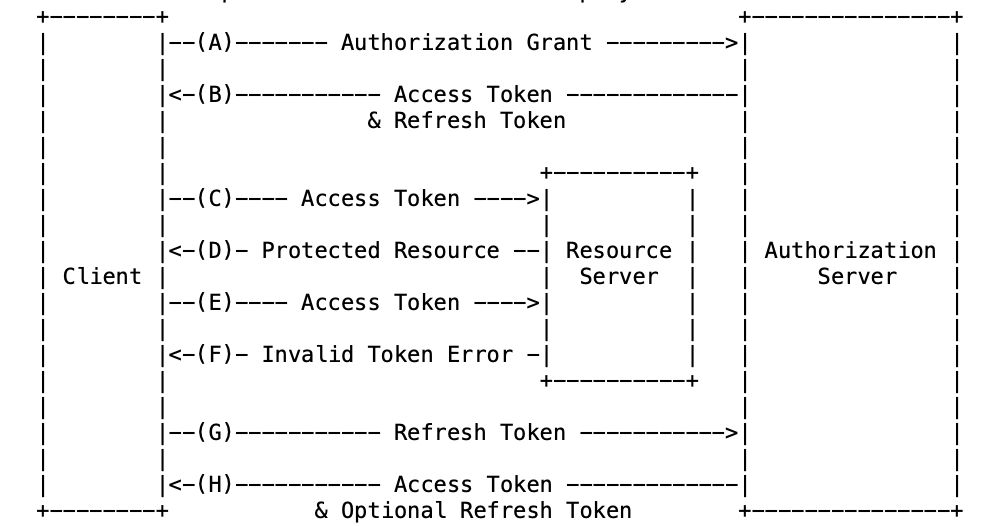
\includegraphics[width=0.5\textwidth]{oauth2.png}
  \caption{OAuth 2.0 verloop}
  \label{fig:example1}
\end{figure}

\subsubsection{Client Types}%
\label{subsubsec:client-types}
Er zijn twee soorten clients die OAuth 2.0 kunnen gebruiken:
\begin{enumerate}[label=\textbf{-}]
    \item Confidential Clients: \\
    Een client die in staat is om de clientgeheimen te beschermen en te vertrouwen op de autorisatieserver om de identiteit van de client te verifiëren. Dit type client is in staat om zowel de autorisatiecode als de Access Token te ontvangen. (bijvoorbeeld een client geïmplementeerd op een beveiligde server met beperkte toegang tot de clientgegevens)
  
    \item Public Clients: \\
    Een client die niet in staat is om de clientgeheimen te beschermen en daarom niet in staat is om de identiteit van de client te verifiëren. Dit type client is alleen in staat om de Access Token te ontvangen. (bijvoorbeeld clients die worden uitgevoerd op het apparaat dat wordt gebruikt door de eigenaar van de bron, zoals een geïnstalleerde native applicatie of een webbrowsergebaseerde applicatie)
\end{enumerate}
Hier zijn enkele applicaties met hun respectievelijke clienttypes:
\begin{enumerate}[label=\textbf{-}]
    \item Web applicatie: \\
    Een webapplicatie die wordt uitgevoerd op een webserver. Dit type client is een confidential client. De clientgeheimen alsook de Access Token worden opgeslagen op de webserver en zijn niet toegankelijk voor de resource-eigenaar.
  
    \item User-Agent gebaseerde applicatie: \\
    Een applicatie die wordt uitgevoerd in de user-agent van de resource-eigenaar, zoals een webbrowser. Dit type client is een public client. De clientgeheimen zijn toegankelijk voor de resource-eigenaar en kunnen niet worden beschermd tegen ongeautoriseerde toegang.
  
    \item Native applicatie: \\
    Een applicatie die wordt uitgevoerd op het apparaat dat wordt gebruikt door de resource-eigenaar, zoals een desktopapplicatie of een mobiele applicatie. Dit type client is een public client. De clientgeheimen zijn toegankelijk voor de resource-eigenaar en kunnen niet worden beschermd tegen ongeautoriseerde toegang.
\end{enumerate}

\subsubsection{Client Authentication}
\label{subsubsec:client-authentication}
De client moet bij elk verzoek niet meer dan één authenticatiemethode gebruiken.

\subsubsection{Endpoints}%
\label{subsubsec:endpoints}
\begin{enumerate}[label=\textbf{-}]
    \item Authorization Endpoint: \\
    Dit endpoint wordt door de clienttoepassing gebruikt om autorisatie van de resource-eigenaar te verkrijgen. Meestal houdt dit in dat de gebruiker wordt omgeleid naar het autorisatie-endpoint van de autorisatieserver, waar hij/zij kan inloggen en machtigingen kan verlenen aan de clienttoepassing. Na het verlenen van autorisatie leidt de autorisatieserver de gebruiker terug naar de clienttoepassing met een autorisatiecode of Access Token.
    \newline
    Een \texttt{response\_type} van ``code'' geeft aan dat de clienttoepassing een autorisatiecode wil ontvangen. Een \texttt{response\_type} van ``token'' geeft aan dat de clienttoepassing een Access Token wil ontvangen.
  
    \item Token Endpoint: \\
    Na het verkrijgen van autorisatie van de eigenaar van de bron, wisselt de clienttoepassing de autorisatiecode uit voor een Access Token door een verzoek naar het token endpoint te sturen. Dit endpoint is verantwoordelijk voor het authenticeren van de client en het uitwisselen van de autorisatiecode voor een Access Token. Het token endpoint wordt door de client gebruikt om een Access Token te verkrijgen door de Authorization Grant of Refresh Token te presenteren.
    \newline
    Met andere woorden is dit endpoint optioneel, omdat de autorisatieserver de Access Token ook kan retourneren in de respons van het autorisatieverzoek. In dit geval is het token endpoint niet nodig.
    \newline
    Men kan dit endpoint ook gebruiken om een nieuwe Access Token te verkrijgen met behulp van een Refresh Token. Dit is handig wanneer de Access Token verloopt of ongeldig wordt.
  
    \item Redirection Endpoint: \\
    Dit is niet bepaald een endpoint, maar het is een cruciaal onderdeel van de OAuth-stroom. Het is de URI waar de autorisatieserver de user-agent (meestal een webbrowser) omleidt nadat de resource-eigenaar toegang tot de clienttoepassing heeft verleend/geweigerd. De redirect-URI bevat doorgaans parameters zoals de autorisatiecode of het Access Token. Wanneer een redirect-URI is opgenomen in een autorisatieverzoek, moet de autorisatieserver de ontvangen waarde vergelijken en matchen met ten minste één van de geregistreerde redirect-URI's (of URI-componenten), als er redirect-URI's zijn geregistreerd. Als de clientregistratie de volledige redirect-URI bevatte, moet de autorisatieserver de twee URI's vergelijken met behulp van eenvoudige string vergelijking. Als de validatie van een autorisatieverzoek mislukt vanwege een ontbrekende, ongeldige of niet-overeenkomende redirect-URI, moet de autorisatieserver de eigenaar van de bron op de hoogte stellen van de fout en moet de user-agent niet automatisch worden omgeleid naar de ongeldige redirect-URI.
  \end{enumerate}

\subsubsection{Authorization request}%
\label{subsubsec:authorization-request}
De client maakt een verzoek naar de autorisatieserver om autorisatie te verkrijgen. Het verzoek bevat de volgende parameters:
\begin{enumerate}[label=\textbf{-}]
    \item response type: \\
    Deze parameter geeft het gewenste responstype aan. De waarde moet ``code'' zijn voor autorisatiecode of ``token'' voor Access Token.
  
    \item client id: \\
    Deze parameter geeft de client-ID van de clienttoepassing aan. De waarde moet overeenkomen met de geregistreerde client-ID van de clienttoepassing.
  
    \item redirect uri: \\
    Deze parameter geeft de URI aan waar de autorisatieserver de gebruiker na autorisatie moet omleiden. De waarde moet overeenkomen met een van de geregistreerde redirect-URI's van de clienttoepassing.
  
    \item scope: \\
    Deze parameter geeft de machtigingen aan die de clienttoepassing wil verkrijgen. De waarde moet een spatiegescheiden lijst van machtigingen zijn.
  
    \item state: \\
    Deze parameter geeft een willekeurige, niet-voorspelbare waarde aan die door de clienttoepassing wordt gegenereerd. De waarde moet worden gebruikt om CSRF-aanvallen te voorkomen.
  \end{enumerate}
  En kan er als volgt uitzien:
  \begin{verbatim}
    GET /authorize?response_type=code&client_id=s6BhdRkqt3&
    state=xyz&redirect_uri=https%3A%2F%2Fclient%2Eexample%2Ecom%2Fcb
    HTTP/1.1
    Host: server.example.com
  \end{verbatim}

\subsubsection{Authorization reponse}%
\label{subsubsec:authorization-reponse}
De autorisatieserver verleent autorisatie aan de clienttoepassing en leidt de gebruiker terug naar de clienttoepassing met een autorisatiecode of Access Token. Het antwoord bevat de volgende parameters:
\begin{enumerate}[label=\textbf{-}]
    \item code: \\
    Deze parameter geeft de autorisatiecode aan die door de autorisatieserver is gegenereerd. De autorisatiecode wordt gebruikt door de clienttoepassing om een Access Token te verkrijgen.
  
    \item state: \\
    Deze parameter geeft de waarde van de state-parameter van het autorisatieverzoek aan. De waarde moet overeenkomen met de waarde die door de clienttoepassing is verstrekt.
  \end{enumerate}
  En kan er als volgt uitzien:
  \begin{verbatim}
    HTTP/1.1 302 Found
    Location: https://client.example.com/cb?code=SplxlOBeZQQYbYS6WxSbIA&state=xyz
  \end{verbatim}

  \subsubsection{Error response}%
  \label{subsubsec:error-response}
  Als het verzoek mislukt vanwege een ontbrekende, ongeldige of niet-overeenkomende redirect-URI, of als de client-ID ontbreekt of ongeldig is, moet de autorisatieserver de eigenaar van de bron op de hoogte stellen van de fout en moet de user-agent niet automatisch omleiden naar de ongeldige redirect-URI.
  
  \subsubsection{Een Access Token vernieuwen}%
  \label{subsubsec:een-access-token-vernieuwen}
  Als de autorisatieserver een Refresh Token aan de client heeft uitgegeven, doet de cliënt een vernieuwingsverzoek aan het token endpoint.
  Indien geldig en geautoriseerd, geeft de autorisatieserver een Access Token uit. Als de verificatie van het verzoek is mislukt of ongeldig is, retourneert de autorisatieserver een foutreactie.
  De autorisatieserver kan een nieuw Refresh Token uitgeven, in welk geval de cliënt het oude Refresh Token moet weggooien en vervangen door het nieuwe Refresh Token. De autorisatieserver kan het oude Refresh Token intrekken nadat een nieuw Refresh Token aan de client is uitgegeven. Als er een nieuw Refresh Token wordt uitgegeven, moet het bereik van het Refresh Token identiek zijn aan dat van het Refresh Token dat door de client in de aanvraag is opgenomen.
  
  \subsubsection{Beveiligingsoverwegingen}
  \label{subsubsec:beveiligingsoverwegingen}
  \begin{enumerate}[label=\textbf{-}]
      \item Client Impersonation: \\
      Een kwaadwillende client kan zich voordoen als een andere client en toegang krijgen tot beschermde bronnen als de nagebootste client er niet in slaagt of niet in staat is zijn clientreferenties vertrouwelijk te houden.
  
      \item Access Tokens: \\
      De autorisatieserver moet ervoor zorgen dat Access Tokens niet door onbevoegde partijen kunnen worden gegenereerd, gewijzigd of geraden om geldige Access Tokens te produceren.
  
      \item Refresh Tokens: \\
      De autorisatieserver moet de binding tussen het Refresh Token en de clientidentiteit verifiëren wanneer de clientidentiteit kan worden geverifieerd. Wanneer clientauthenticatie niet mogelijk is, moet de autorisatieserver andere middelen inzetten om misbruik van Refresh Token te detecteren. De autorisatieserver zou bijvoorbeeld Refresh Token rotatie kunnen gebruiken, waarbij een nieuw Refresh Token wordt uitgegeven bij elke vernieuwingsreactie van het Access Token. Het vorige Refresh Token wordt ongeldig gemaakt, maar behouden door de autorisatieserver. Als een Refresh Token wordt aangetast en vervolgens door zowel de aanvaller als de legitieme client wordt gebruikt, zal een van hen een ongeldig Refresh Token presenteren, dat de autorisatieserver op de hoogte stelt van de inbreuk. De autorisatieserver moet ervoor zorgen dat Refresh Tokens niet door onbevoegde partijen kunnen worden gegenereerd, gewijzigd of geraden dat ze geldige Refresh Tokens produceren.
  
      \item Request Confidentiality: \\
      Access Tokens, Refresh Tokens, wachtwoorden voor resource-eigenaren en klantreferenties moeten niet openbaar worden verzonden. De parameters ``state'' en ``scope'' moeten geen gevoelige klant- of resource-eigenaarinformatie in platte tekst bevatten, omdat deze via onveilige kanalen kunnen worden verzonden of onveilig kunnen worden opgeslagen.
  \end{enumerate}


  \subsection{OAuth 2.0 voor Native Apps}%
  \label{subsec:oauth-2.0-voor-native-apps}
  \autocite{Denniss2017}
  Een native app is een app die door de gebruiker op zijn apparaat wordt geïnstalleerd, in tegenstelling tot een webapp die alleen in de browsercontext wordt uitgevoerd. Apps die zijn geïmplementeerd met behulp van webgebaseerde technologie maar worden gedistribueerd als een native app, de zogenaamde ``hybride apps'', worden voor het doel van deze specificatie beschouwd als gelijkwaardig aan native apps.
  OAuth 2.0-autorisatieverzoeken van native apps worden het best, en het liefst alleen, gedaan via externe user-agents, voornamelijk de browser van de gebruiker. Het andere alternatief is het gebruik van ingebedde user-agents. Deze aanpak heeft veel nadelen, waaronder het feit dat de host-app gebruikersgegevens en cookies kan kopiëren en dat de gebruiker zich in elke app helemaal opnieuw moet authenticeren. Autorisatieverzoeken voor native apps die de browser gebruiken, zijn veiliger en kunnen profiteren van de authenticatiestatus van de gebruiker. Door de bestaande authenticatiesessie in de browser te kunnen gebruiken, is eenmalige aanmelding (SSO) mogelijk, omdat gebruikers zich niet telkens opnieuw hoeven te authenticeren bij de autorisatieserver wanneer ze een nieuwe app gebruiken.
  Om deze best practices te ondersteunen, dienen bepaalde OAuth-serverimplementaties die vertrouwen op alle clients als vertrouwelijk (confidential) voor het web, openbare (public) native app-clients en hun bijbehorende soorten redirect-URI's te erkennen.
  \begin{figure}[h]
    \centering
    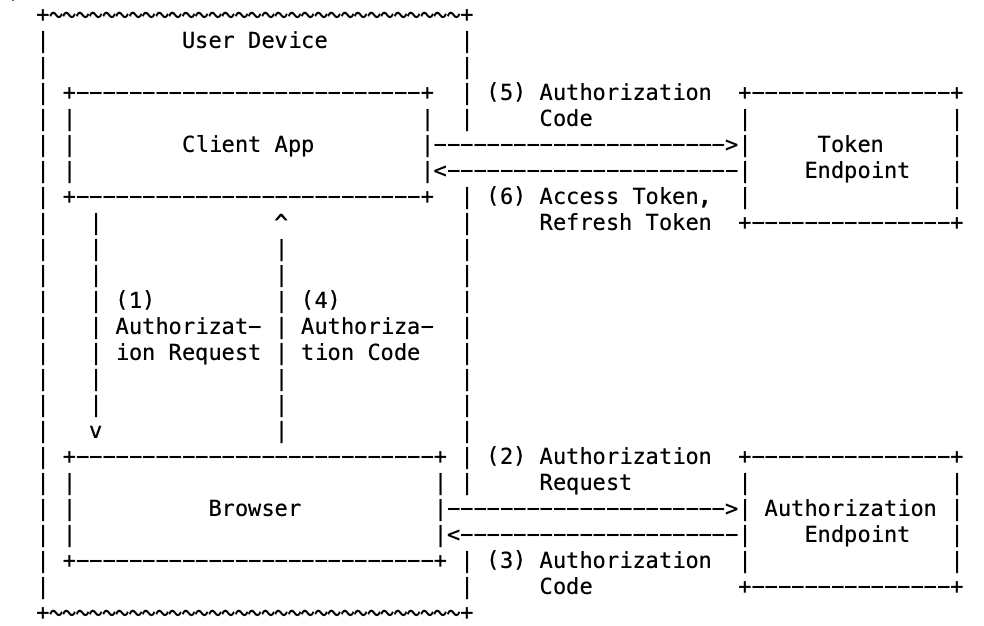
\includegraphics[width=0.5\textwidth]{oauth2_native.png}
    \caption{OAuth 2.0 verloop in native apps}
    \label{fig:example2}
  \end{figure}
  \newline
  Dit wordt bereikt door het autorisatieverzoek in de browser te openen en een redirect-URI te gebruiken die het autorisatieantwoord terugstuurt naar de native app.
  \newline
  \newline
  Het ontvangen van de Autorisatiereactie in een Native App gebeurt ook via een redirect URI, er zijn verschillende opties:
  \newline
  - Omleiding van URI-schema voor privégebruik: nadat de auth-server het verzoek heeft voltooid, wordt deze omgeleid naar de omleidings-URI van de client, com.example.app:/oauth2redirect/example-provider, dit resulteert erin dat het besturingssysteem de native app start en de URI als startparameter.
  \newline
  - Geclaimde 'https'-schema-URI-omleiding: https://app.example.com/oauth2redirect/example-provider, door de app geclaimde 'https'-schema-omleidings-URI's hebben enkele voordelen vergeleken met andere native app-omleidingsopties, omdat de identiteit van de de bestemmingsapp wordt door het besturingssysteem gegarandeerd aan de autorisatieserver. Om deze reden moeten native apps deze waar mogelijk boven de andere opties gebruiken.
  \newline
  - Loopback Interface Redirection: http://127.0.0.1:51004/oauth2redirect/example-provider, voornamelijk voor desktop-apps die een poort op de loopback-netwerkinterface kunnen openen zonder speciale machtigingen nodig te hebben, kunnen de loopback-interface gebruiken om de OAuth te ontvangen omleiden.

  
  \subsection{OAuth 2.0: Bearer Token gebruik}%
  \label{subsec:oauth-2.0-bearer-token-gebruik}
  OAuth 2.0 bearer tokens kunnen worden gebruikt in HTTP-verzoeken om toegang te krijgen tot beveiligde bronnen \autocite[p.~{Section 1.0}]{Jones2012}.
  Een bearer token is een token dat kan worden gebruikt door iedereen die eigenaar is van het token, zonder dat er bewijs nodig is van het bezit van cryptografisch materiaal \autocite[p.~{Section 1.2}]{Jones2012}.
  Er worden drie manieren beschreven om een bearer token in een aanvraag op te nemen: in de Authorization-header, als een formuliergecodeerde body-parameter of als een URI-queryparameter \autocite[p.~{Section 2.1}]{Jones2012}. Als een verzoek mislukt, moet de bronserver een 401-statuscode en een foutcode retourneren, zoals 'invalid\verb|_|request', 'invalid\verb|_|token' of 'insufficient\verb|_|scope' \autocite[p.~{Section 3.0}]{Jones2012}.
  Het gebruik van TLS, het valideren van certificaten, het uitgeven van tokens voor de korte termijn en het niet opslaan van tokens in cookies zijn elk sterk aanbevolen \autocite[p.~{Section 5.0}]{Jones2012}.


  \subsection{JWT huidige Best Practices}%
  \label{subsec:jwt-huidige-best-practices}
  Deze sectie lijst de bekende en mogelijke problemen op met JWT-implementaties en -inzet. Elk probleem wordt gevolgd door verwijzingen naar een of meer maatregelen om deze problemen te verhelpen.
  \begin{enumerate}[label=\textbf{-}]
      \item Zwakke Handtekeningen en Onvoldoende Validatie van Handtekeningen
      \item Zwakke Symmetrische Sleutels: Deze zijn even onveilig als makkelijk te onthouden wachtwoorden.
      \item Onjuiste Samenstelling van Encryptie en Handtekening: Sommige bibliotheken die een JWE-versleutelde JWT ontcijferen om een JWS-ondertekend object te verkrijgen, valideren niet altijd de interne handtekening.
      \item Plaintext lek door Analyse van Cijfertekstlengte: Veel encryptiealgoritmen lekken informatie over de lengte van de oorspronkelijke tekst.
      \item Onveilig Gebruik van Elliptische Curve-Encryptie
      \item Veelvoud van JSON-coderingen
      \item Substitutieaanvallen: Dit zijn aanvallen waarbij een ontvanger een JWT krijgt die voor hem bedoeld was en probeert deze te gebruiken bij een andere ontvanger waarvoor die JWT niet bedoeld was.
      \item Kruis-JWT-verwarring: Gevallen voorkomen waarin JWT-tokens die zijn uitgegeven voor een bepaald doel, worden ondermijnd en gebruikt voor een ander doel.
      \item Indirecte Aanvallen op de Server
  \end{enumerate}
  Best Practices
  \begin{enumerate}[label=\textbf{-}]
    \item Voer algoritmeverificatie uit: Zorg ervoor dat de algoritmen die worden gebruikt voor het ondertekenen en versleutelen van JWT's veilig zijn.
    \item Gebruik geschikte algoritmen: Gebruik veilige algoritmen voor het ondertekenen en versleutelen van JWT's.
    \item Valideer alle cryptografische bewerkingen: Zorg ervoor dat alle cryptografische bewerkingen correct worden uitgevoerd.
    \item Valideer cryptografische invoer: Zorg ervoor dat alle invoer voor cryptografische bewerkingen correct is. Dit omvat het valideren van de lengte van de invoer, het controleren van de invoer op ongeldige tekens en het valideren van de invoer tegen een lijst met bekende sleutels.
    \item Zorg ervoor dat cryptografische sleutels voldoende entropie hebben: Entropie is een maat voor de onvoorspelbaarheid van een reeks gegevens.
    \item Vermijd compressie van coderingsinvoer: Compressie van coderingsinvoer kan leiden tot lekken van informatie over de oorspronkelijke tekst.
    \item Gebruik UTF-8: Zorg ervoor dat alle tekst die wordt gebruikt in JWT's wordt gecodeerd in UTF-8.
    \item Valideer de uitgever en het onderwerp: Issuer en Subject
    \item Gebruik en valideer doelgroep: Audience
    \item Vertrouw ontvangen claims niet
    \item Gebruik expliciet typen
    \item Gebruik wederzijds exclusieve validatieregels voor verschillende soorten JWT's
  \end{enumerate}
  \autocite{Sheffer2020}


  \subsection{OpenID Connect}%
  \label{subsec:openid-connect}
  OpenID Connect is een identiteitslaag bovenop OAuth 2.0, dat wordt gebruikt voor authenticatie. Het is een eenvoudige identiteitslaag die bovenop OAuth 2.0 is gebouwd en die de authenticatie van gebruikers mogelijk maakt. OpenID Connect biedt een eenvoudige manier om gebruikers te verifiëren en toegang te verlenen tot applicaties en services. Het maakt gebruik van JSON Web Tokens (JWT's) om claims over gebruikers te verstrekken en om gebruikers te verifiëren. OpenID Connect is ontworpen om eenvoudig te implementeren en te gebruiken en biedt een veilige en betrouwbare manier om gebruikers te verifiëren en toegang te verlenen tot applicaties en services.
  \newline
  \newline
  OpenID Connect biedt een aantal voordelen ten opzichte van traditionele authenticatiemethoden, waaronder:
  \begin{enumerate}[label=\textbf{-}]
      \item Eenvoudige implementatie: OpenID Connect is eenvoudig te implementeren en te gebruiken en biedt een gestandaardiseerde manier om gebruikers te verifiëren en toegang te verlenen tot applicaties en services.
      \item Veilige en betrouwbare authenticatie: OpenID Connect maakt gebruik van JSON Web Tokens (JWT's) om claims over gebruikers te verstrekken en om gebruikers te verifiëren. Dit biedt een veilige en betrouwbare manier om gebruikers te verifiëren en toegang te verlenen tot applicaties en services.
      \item Flexibiliteit: OpenID Connect biedt een flexibele manier om gebruikers te verifiëren en toegang te verlenen tot applicaties en services. Het ondersteunt verschillende authenticatiemethoden en kan worden gebruikt in een breed scala van toepassingen.
      \item Schaalbaarheid: OpenID Connect is schaalbaar en kan worden gebruikt in grote en complexe omgevingen. Het biedt een betrouwbare manier om gebruikers te verifiëren en toegang te verlenen tot applicaties en services.
  \end{enumerate}
  \autocite{Sakimura2014}


  \subsection{Biometrische authenticatie}%
  \label{subsec:biometrische-authenticatie}
  Biometrische authenticatie is een methode voor het verifiëren van de identiteit van een persoon op basis van fysieke of gedragskenmerken. Het maakt gebruik van biometrische gegevens zoals vingerafdrukken, gezichtsherkenning en irisscans om gebruikers te verifiëren en toegang te verlenen tot systemen, applicaties en gegevens. Biometrische authenticatie biedt een veilige en gebruiksvriendelijke manier om gebruikers te verifiëren en biedt bescherming tegen identiteitsdiefstal en fraude. Het wordt gebruikt in een breed scala van toepassingen, waaronder mobiele apparaten, computers, toegangscontrolesystemen en financiële transacties. Biometrische authenticatie wordt steeds populairder vanwege de groeiende behoefte aan veilige en gemakkelijke manieren om gebruikers te verifiëren en hun identiteit te beschermen. Het biedt een effectieve manier om de beveiliging van systemen en gegevens te verbeteren en biedt een betere gebruikerservaring dan traditionele wachtwoordgebaseerde methoden. Biometrische authenticatie wordt beschouwd als een van de meest veilige en betrouwbare methoden voor het verifiëren van de identiteit van een persoon en wordt steeds vaker gebruikt in verschillende sectoren, waaronder banksector, gezondheidszorg, overheid en bedrijfsleven.
  \newline
  \newline
  Misbruik van traditionele beveiligings maatregelen, zoals wachtwoorden, heeft geleid tot de ontwikkeling van biometrische authenticatie als een veiligere en betrouwbaardere methode voor het verifiëren van de identiteit van een persoon. Biometrische gegevens zijn uniek voor elke persoon en kunnen niet, in het slechtste geval moeilijk, worden nagemaakt of gestolen, waardoor ze een effectieve manier zijn om de identiteit van een persoon te verifiëren.
  
  \subsubsection{Gezichtsherkenning}%
  \label{subsubsec:gezichtsherkenning}
  Deze systemen gebruiken de unieke gelaatstrekken van een persoon om deze te identificeren. Het wordt op verschillende plaatsen gebruikt, zoals op smartphones, creditcardbetalingen en bij wetshandhaving.
  
  \subsubsection{Vingerafdrukherkenning}%
  \label{subsubsec:vingerafdrukherkenning}
  Vingerafdrukauthenticatie maakt gebruik van de unieke vingerafdruk van een persoon om zijn identiteit te verifiëren. Het kan worden gebruikt om alles te beveiligen, van mobiele apparaten tot auto's en zelfs gebouwen, waardoor het de meest wijd verspreide biometrische authenticatietechnologie is.
  
  \subsubsection{Oogherkenning}%
  \label{subsubsec:oogherkenning}
  Oogherkenning maakt gebruik van het unieke patroon van iemands iris of netvlies om iemand te identificeren. Omdat dit type biometrische authenticatie moeilijker te implementeren is, komt het minder vaak voor dan de andere soorten biometrische authenticatieopties. Een irisscan vereist een infraroodlichtbron, een camera die IR kan zien en minimale lichtvervuiling om nauwkeurigheid te garanderen. Hoewel het uitdagingen met zich meebrengt, is het een van de meest nauwkeurige biometrische authenticatiesystemen die beschikbaar zijn als aan deze voorwaarden wordt voldaan. Oogherkenning wordt over het algemeen gebruikt in situaties waarin de veiligheid het meest kritisch is, zoals bij nucleaire onderzoeksfaciliteiten, enz.
  
  \subsubsection{Spraakherkenning}%
  \label{subsubsec:spraakherkenning}
  Spraakherkenning maakt gebruik van de toon, toonhoogte en frequenties die uniek zijn voor een individu om deze te authenticeren. Dit is de meest gebruikte biometrie om gebruikers te verifiëren wanneer ze contact opnemen met een callcenter voor klantenservice (bijvoorbeeld online bankieren).
  
  \subsubsection{Gangherkenning}%
  \label{subsubsec:gangherkenning}
  Gangherkenning authenticeert door gebruik te maken van de manier waarop iemand loopt om hem/haar te identificeren. Elke persoon loopt een beetje anders, dus de manier waarop iemand de ene voet voor de andere zet, is een effectieve manier om zijn identiteit te verifiëren. Op dit moment is het geen gebruikelijke vorm van authenticatie, maar de verwachting is dat dit steeds gebruikelijker zal worden naarmate toekomstige vormen van authenticatie populairder worden.
  
  \subsubsection{Aderherkenning}%
  \label{subsubsec:aderherkenning}
  Bij aderherkenning wordt gebruik gemaakt van het patroon van de bloedvaten in de hand of vinger van een persoon om deze te identificeren. Bij dit type biometrische authenticatie wordt gebruik gemaakt van infraroodlicht om de aderen onder de huid van uw handen of vingers in kaart te brengen. Aderherkenning is uiterst nauwkeurig, meer dan netvlies-/irisherkenning.
  
  \subsubsection{Multimodale biometrische authenticatie}%
  \label{subsubsec:multimodale-biometrische-authenticatie}
  Eerst moet men begrijpen wat een unimodaal biometrisch authenticatie systeem is. Dit is een systeem dat verifieert op basis van 1 biometrische methode, het is dan uiteraard niet verwondelijk dat dit soort systemen heel kwetsbaar zijn voor spoofing.
  \newline
  \newline
  Dit is waar multimodale biometrische authenticatie in beeld komt. Het is een aanpak waarin meerdere biometrische eigenschappen worden gebruikt om de identiteit van een persoon te verifiëren. Dit kan bijvoorbeeld een combinatie zijn van gezichtsherkenning en vingerafdrukherkenning. Door meerdere biometrische eigenschappen te combineren, wordt de nauwkeurigheid van het authenticatiesysteem verhoogd en wordt het moeilijker voor aanvallers om het systeem te misleiden. Multimodale biometrische authenticatie wordt steeds populairder vanwege de groeiende behoefte aan veilige en betrouwbare authenticatiesystemen.
  
  \subsubsection{De voordelen van biometrische authenticatie}%
  \label{subsubsec:de-voordelen-van-biometrische-authenticatie}
  \begin{enumerate}[label=\textbf{-}]
    \item Identiteitsverzekering: \\
    Biometrische identificatie biedt de antwoorden op “iets wat een persoon heeft en is” en helpt de identiteit te verifiëren. Biometrische authenticatie zorgt voor meer zekerheid voor eindgebruikers. De geavanceerde software laat providers weten dat een persoon is wie ze beweren te zijn door middel van een tastbare, reële eigenschap. Zelfs als een cyberaanvaller het wachtwoord van een gebruiker of het antwoord op zijn beveiligingsvraag kent, is het onmogelijk dat hij of zij een vingerafdruk of irisscan kan dupliceren.
  
    \item Gebruiksgemak: \\
    Hoewel biometrische authenticatie meer technisch van aard is met betrekking tot het interne proces, is het over het algemeen gemakkelijk en snel vanuit het oogpunt van de gebruiker. Door een vingerafdrukscanner te gebruiken om een account te ontgrendelen of gezichtsherkenning, vermindert u het aantal keren dat u moet inloggen met een lang wachtwoord dat meerdere speciale tekens bevat die u waarschijnlijk uiteindelijk zult vergeten.
  
    \item Fraudedetectie: \\
    Biometrie is bijna onmogelijk te repliceren. Ze zijn moeilijk te repliceren en te stelen, en de kans is slechts ongeveer 1 op 64 miljard \autocite{Baker2021} \autocite{Lee2013} dat jouw vingerafdruk precies overeenkomt met die van iemand anders. Het is zeer onwaarschijnlijk dat een hacker toegang krijgt tot alles dat met biometrie is beveiligd.
  \end{enumerate}
  
  \subsubsection{De nadelen van biometrische authenticatie}%
  \label{subsubsec:de-nadelen-van-biometrische-authenticatie}
  \begin{enumerate}[label=\textbf{-}]
    \item Hackbaar: \\
    Biometrie kan nog steeds worden gehackt. Bedrijven en overheden die de persoonlijke gegevens van gebruikers verzamelen en opslaan, worden voortdurend bedreigd door hackers. Als ze echter het slachtoffer worden van een datalek, zijn biometrische gegevens onvervangbaar en moeten organisaties zorgvuldig omgaan met de biometrische gegevens van gebruikers.
  
    \item Gedeeltelijke overeenkomsten: \\
    De meeste gangbare biometrische authenticatiemethoden zijn afhankelijk van gedeeltelijke informatie om de identiteit van een gebruiker te verifiëren. Tijdens het registratieproces voor het registreren van uw vingerafdruk worden bijvoorbeeld gegevens van uw gehele afdruk gebruikt en omgezet in gegevens. Tijdens toekomstige authenticatie zijn echter slechts gedeeltelijke vingerafdrukgegevens nodig om uw identiteit te verifiëren, zodat het steeds sneller gaat.
  
    \item Onnauwkeurigheid: \\
    Biometrische authenticatie is niet perfect en kan fouten maken bij het identificeren van gebruikers. Dit kan leiden tot frustratie bij gebruikers en kan de veiligheid van het systeem in gevaar brengen. Het is belangrijk om de nauwkeurigheid van biometrische authenticatie te evalueren voordat u het implementeert.
  \end{enumerate}


  \subsection{WebAuthn}%
  \label{subsec:webauthn}
  WebAuthn is een W3C-specificatie die een webstandaard biedt voor biometrische authenticatie. Het is bedoeld om een veilige en gebruiksvriendelijke manier te bieden om gebruikers te verifiëren zonder dat ze wachtwoorden hoeven te onthouden. WebAuthn maakt gebruik van openbare en privésleutels om gebruikers te verifiëren en biedt een veilige manier om in te loggen op websites en applicaties. Het maakt gebruik van biometrische gegevens zoals vingerafdrukken, gezichtsherkenning en irisscans om gebruikers te verifiëren en biedt een veilige manier om in te loggen op websites en applicaties. WebAuthn is ontworpen om de beveiliging van online accounts te verbeteren en gebruikers te beschermen tegen phishingaanvallen en andere vormen van cybercriminaliteit. Het is een open standaard die wordt ondersteund door alle grote webbrowsers en platformen en wordt gebruikt door bedrijven over de hele wereld om hun online accounts te beveiligen. WebAuthn is een belangrijke stap voorwaarts in de strijd tegen cybercriminaliteit en biedt een veilige en gebruiksvriendelijke manier om gebruikers te verifiëren en hun online accounts te beschermen.
  
  
  
  \section{Auth aanbieders}%
  \label{sec:auth-aanbieders}
  In deze sectie worden enkele van de belangrijkste aanbieders van authenticatiediensten besproken, waaronder Auth0, TrustBuilder en meer. Deze aanbieders bieden een reeks diensten en tools om ontwikkelaars te helpen bij het implementeren van authenticatie en autorisatie in hun applicaties. Ze bieden ook ondersteuning voor verschillende authenticatieprotocollen, waaronder OAuth 2.0 en OpenID Connect, en bieden een reeks functies om ontwikkelaars te helpen bij het beheren van gebruikersidentiteiten en toegangscontrole.
  De reden waarom we aanbieders bespreken en vergelijken is om inzicht te krijgen in wat er momenteel wordt aangeboden op de markt, zodat de must haves kunnen worden bepaald voor de ontwikkeling van een eigen authenticatieservice of light weight instance (zie later).
  
  
  \subsection{Auth0}%
  \label{subsec:auth0}
  Auth0 is a popular Identity as a Service (IDaaS) platform that provides authentication and authorization services. It supports various identity providers, social logins, and multi-factor authentication. Auth0 offers a range of features, including user management, single sign-on, and passwordless authentication. It also provides SDKs and APIs for integrating authentication into web and mobile applications. Auth0 is widely used by developers and organizations to secure their applications and protect user identities. It is known for its ease of use, scalability, and security features.
  
  
  \subsection{TrustBuilder}%
  \label{subsec:trustbuilder}
  TrustBuilder is een Belgisch bedrijf dat gespecialiseerd is in Identity and Access Management (IAM) oplossingen. Het doel van TrustBuilder is om organisaties te helpen bij het beheren van de toegangscontrole tot hun digitale middelen, zoals applicaties, gegevens en systemen, op een veilige en efficiënte manier. Het biedt oplossingen voor authenticatie, autorisatie en het beheer van identiteiten, waardoor organisaties de beveiliging kunnen versterken en tegelijkertijd een naadloze gebruikerservaring kunnen bieden. TrustBuilder richt zich voornamelijk op bedrijven in verschillende sectoren, waaronder financiële dienstverlening, gezondheidszorg, overheid en retail.
  
  
  \subsection{Andere}%
  \label{subsec:andere}
  Naast Auth0 en TrustBuilder zijn er nog andere aanbieders van authenticatiediensten, waaronder:
  \begin{enumerate}[label=\textbf{-}]
    \item Okta: Okta is een toonaangevende aanbieder van Identity and Access Management (IAM) oplossingen. Het biedt een reeks diensten en tools om organisaties te helpen bij het beheren van gebruikersidentiteiten en toegangscontrole. Het ondersteund Single Sign-On (SSO), Multi-Factor Authentication (MFA), adaptieve authenticatie, API-toegangsbeheer, lifesyclebeheer van gebruikers en groepen en meer.
    \item Firebase Authentication: Firebase Authentication is een dienst van Google die ontwikkelaars helpt bij het implementeren van authenticatie in hun applicaties. Het biedt ondersteuning voor verschillende authenticatiemethoden, waaronder e-mail en wachtwoord, telefoonnummer, Google, Facebook, Twitter en GitHub.
    \item Amazon Cognito: Amazon Cognito is een dienst van Amazon Web Services (AWS) die ontwikkelaars helpt bij het implementeren van authenticatie en autorisatie in hun applicaties. Het biedt ondersteuning voor gebruikersregistratie, inloggen, groepen, rollen en toegangsbeheer.
    \item Microsoft Azure Active Directory: Azure Active Directory is een dienst van Microsoft die ontwikkelaars helpt bij het implementeren van authenticatie en autorisatie in hun applicaties. Het biedt ondersteuning voor Single Sign-On (SSO), Multi-Factor Authentication (MFA), en kan worden geïntegreerd met verschillende toepassingen van Microsoft en derden.
    \item Google Identity Platform: Google Identity Platform biedt authenticatie- en autorisatieservices. Het ondersteunt Google Sign-In, OAuth 2.0 en OpenID Connect voor integratie met de identiteitsservices van Google.
  \end{enumerate}



\section{Light weight OAuth 2.0 Docker image}%
\label{sec:light-weight-oauth-2.0-docker-image}
Uit vorige onderzoeken kan men concluderen dat auth al veel verder is geëvolueerd dan men had kunnen verwachten. Er zijn veel aanbieders die een breed scala aan diensten aanbieden, van authenticatie tot autorisatie en alles daartussenin. Het is duidelijk dat het implementeren van een eigen auth-service een enorme taak is en dat het waarschijnlijk niet de moeite waard is, maar dit zou wel een enorme leerervaring zijn.
\newline
\newline
Het volgende dat onderzocht werd was of er light weight instances bestaan, zoals bijvoorbeeld een Docker Image, die OAuth 2.0 implementeren. Dit zou een goede oplossing zijn voor een kleinere applicatie die geen behoefte heeft aan de uitgebreide diensten die Auth0 en TrustBuilder aanbieden. Het zou ook een goede oplossing zijn voor een ontwikkelaar die wil leren hoe OAuth 2.0 werkt en hoe het kan worden geïmplementeerd in hun eigen applicatie, zonder af te hangen van een derde partij.
\newline
\newline
Uit een volgend onderzoek bleek dat er al een aantal Docker Images bestonden die OAuth 2.0 implementeert, namelijk Keycloak, Hydra, Oathkeeper en meer.

%%=============================================================================
%% Methodologie
%%=============================================================================

\chapter{\IfLanguageName{dutch}{Methodologie}{Methodology}}%
\label{ch:methodologie}

%% TODO: In dit hoofstuk geef je een korte toelichting over hoe je te werk bent
%% gegaan. Verdeel je onderzoek in grote fasen, en licht in elke fase toe wat
%% de doelstelling was, welke deliverables daar uit gekomen zijn, en welke
%% onderzoeksmethoden je daarbij toegepast hebt. Verantwoord waarom je
%% op deze manier te werk gegaan bent.
%% 
%% Voorbeelden van zulke fasen zijn: literatuurstudie, opstellen van een
%% requirements-analyse, opstellen long-list (bij vergelijkende studie),
%% selectie van geschikte tools (bij vergelijkende studie, "short-list"),
%% opzetten testopstelling/PoC, uitvoeren testen en verzamelen
%% van resultaten, analyse van resultaten, ...
%%
%% !!!!! LET OP !!!!!
%%
%% Het is uitdrukkelijk NIET de bedoeling dat je het grootste deel van de corpus
%% van je bachelorproef in dit hoofstuk verwerkt! Dit hoofdstuk is eerder een
%% kort overzicht van je plan van aanpak.
%%
%% Maak voor elke fase (behalve het literatuuronderzoek) een NIEUW HOOFDSTUK aan
%% en geef het een gepaste titel.


\section{Vergelijkingscriteria Auth aanbieders}%
\label{sec:vergelijkingscriteria-auth-aanbieders}

\begin{enumerate}
  \item Hoofd functionaliteit: Wat zijn de belangrijkste functionaliteiten?
  \item Ontwikkelaars ervaring: Wat ervaren ontwikkelaars? Hoe gemakkelijk is het te gebruiken? (Documentatie, SDKs, integraties, \ldots)
  \item Integratie mogelijkheden: Hoe gemakkelijk integreert het met tech stacks, frameworks, gerelateerde producten, \ldots?
  \item Use Cases: Waarom en wanneer gebruik je de auth aanbieder het best?
\end{enumerate}


\section{Auth aanbieders vergelijken}%
\label{sec:auth-aanbieders-vergelijken}
Op basis van de eerder genoemde criteria, werden de volgende Docker Images verder besproken en vergeleken: Auth0, Okta, Firebase Authentication en Amazon Cognito.
\begin{enumerate}
  \item Hoofd functionaliteit:
  \begin{itemize}
    \item Auth0 biedt een uitgebreide ondersteuning voor diverse identiteitsproviders, waaronder sociale logins en bedrijfsverbindingen, waardoor gebruikers een naadloze en veelzijdige inlogervaring hebben. Het platform gaat verder dan standaard beveiligingsmaatregelen door multi-factor authenticatie (MFA) en anomaly detectie te bieden, waardoor extra bescherming wordt geboden tegen ongeautoriseerde toegangspogingen. Bovendien kunnen bedrijven de inlog- en aanmeldingspagina's aanpassen aan hun eigen huisstijl, wat bijdraagt aan een consistente merkervaring voor gebruikers. Met de rules engine van Auth0 kunnen organisaties op maat gemaakte authenticatie- en autorisatielogica implementeren, waardoor ze flexibel kunnen inspelen op specifieke beveiligingsbehoeften en zakelijke vereisten.
    \item Okta staat bekend om zijn uitgebreide oplossingen op het gebied van identity and access management (IAM), waaronder een scala aan functionaliteiten die organisaties helpen bij het beheren van gebruikersidentiteiten en toegangsrechten. Enkele van de prominente kenmerken zijn Single Sign-On (SSO), wat gebruikers in staat stelt om met één set inloggegevens toegang te krijgen tot meerdere applicaties, adaptieve authenticatie die dynamisch reageert op verschillende risiconiveaus, en multi-factor authenticatie voor extra beveiligingslagen. Daarnaast biedt Okta ook API Access Management om de beveiliging van API's te waarborgen, en levenscyclusbeheerfunctionaliteiten voor het efficiënt beheren van gebruikersaccounts en groepen binnen een organisatie.
    \item Firebase Authentication is een cruciaal onderdeel van de uitgebreide Firebase-suite. Het biedt een breed scala aan authenticatiemogelijkheden voor diverse platforms, waaronder web, mobiel en server. Met ondersteuning voor inloggen via e-mail/wachtwoord, sociale media en telefoonnummerverificatie, biedt het een veelzijdige oplossing voor gebruikersidentificatie. Bovendien kan Firebase Authentication naadloos worden geïntegreerd met andere services binnen het Firebase-ecosysteem, waardoor ontwikkelaars een gestroomlijnde en consistente ontwikkelingservaring krijgen.
    \item Amazon Cognito is een uitgebreide identiteitsservice die wordt beheerd door AWS (Amazon Web Services). Het biedt een scala aan functionaliteiten, waaronder gebruikersregistratie en -aanmelding, multi-factor authenticatie en veilige toegangscontrole. Bovendien integreert het naadloos met AWS Identity and Access Management (IAM), waardoor gedetailleerde controle over toegangsrechten mogelijk is.
  \end{itemize}
  
  \item Ontwikkelaars ervaring:
  \begin{itemize}
    \item Auth0 heeft goed gedocumenteerde API's en SDK's voor verschillende platformen en uitgebreide reeks functies voor ontwikkelaars, inclusief hooks voor het aanpassen van workflows.
    \item Okta heeft goed gedocumenteerde API's en SDK's voor makkelijke integratie mogelijk te maken omdat het kant-en-klare integraties biedt met populaire applicaties.
    \item Firebase Authentication biedt naadloze integratie met andere Firebase-services, alsook vereenvoudigde SDK's voor populaire platformen.
    \item Amazon heeft goed gedocumenteerde API's en SDK's voor verschillende programmeertalen met naadloze integratie met andere AWS-services.
  \end{itemize}
  
  \item Integratie mogelijkheden:
  \begin{itemize}
    \item Auth0 maakt moeiteloze integratie met diverse technologieën en frameworks mogelijk. Het biedt uitgebreide ondersteuning voor Single Sign-On (SSO) voor alle applicaties, waardoor gebruikers moeiteloos toegang krijgen zonder herhaaldelijk in te loggen.
    \item Okta kan goed worden geïntegreerd met verschillende cloudservices en bedrijfsapplicaties. Het biedt robuuste ondersteuning voor SSO en toegangsbeheer.
    \item Firebase Authentication is ontworpen voor integratie met Firebase-aangedreven applicaties. Geschikt voor projecten gebouwd op het Firebase-platform.
    \item Amazon Cognito integreert soepel met andere AWS-services en cloud-native applicaties. Geschikt voor projecten binnen het AWS-ecosysteem.
  \end{itemize}
  
  \item Use Cases:
  \begin{itemize}
    \item Auth0 is geschikt voor een breed scala aan toepassingen, van kleine projecten tot grote bedrijfsoplossingen.
    \item Okta is zeer geschikt voor ondernemingen die een uitgebreide IAM-oplossing nodig hebben met de nadruk op beveiliging en compliance.
    \item Firebase Authentication is ideaal voor ontwikkelaars die aan projecten binnen het Firebase-ecosysteem werken.
    \item Amazon Cognito is ideaal voor applicaties die worden gehost op AWS en biedt schaalbaarheid en nauwe integratie met andere AWS-services.
  \end{itemize}
\end{enumerate}



\section{Vergelijkingscriteria OAuth 2.0 Docker Image's}%
\label{sec:vergelijkingscriteria-oauth2-docker-image}

\begin{enumerate}
  \item Gebruiksgemak en configuratie: Hoe gemakkelijk is het om de Docker-image in te stellen en te configureren voor je specifieke gebruiksscenario? Worden er duidelijke instructies geleverd?

  \item Ondersteunde OAuth 2.0-functies: Controleer welke functies van het OAuth 2.0 protocol worden ondersteund door de verschillende implementaties. Dit kan onder meer autorisatiecodes, impliciete access tokens, client credentials en refresh tokens omvatten.
  
  \item Ondersteuning voor andere protocollen: Sommige auth server implementaties ondersteunen naast OAuth 2.0 ook andere protocollen zoals OpenID Connect. Het kan handig zijn om te beoordelen welke protocollen worden ondersteund als je behoeften hebt die verder gaan dan alleen OAuth 2.0.
  
  \item Schaalbaarheid en prestaties: Hoe schaalbaar is de auth server? Kan het omgaan met een groot aantal gelijktijdige gebruikers en verzoeken? Zijn er prestatie benchmarks beschikbaar?
  
  \item Aanpasbaarheid en uitbreidbaarheid: Kun je de functionaliteit van de auth server aanpassen of uitbreiden met behulp van plugins of aangepaste code?
  
  \item Documentatie en community ondersteuning: Is er uitgebreide documentatie beschikbaar voor de Docker-image en de bijbehorende auth server? Is er een actieve community waar je vragen kunt stellen en ondersteuning kunt krijgen?
  
  \item Beveiligingsfuncties: Welke beveiligingsfuncties biedt de auth server? Wordt er bijvoorbeeld ondersteuning geboden voor multifactor authenticatie, JWT verificatie of integratie met externe identiteitsproviders?
  
  \item Onderhoud en updates: Wordt de Docker-image regelmatig bijgewerkt met bug fixes en beveiliging patches? Hoe actief is de ontwikkeling van de auth server?
  
  \item Beschikbaarheid van integraties: Controleer of de auth server integraties biedt met populaire frameworks, bibliotheken en platforms die je gebruikt in je applicatie stack.
  
  \item Kosten en licentie: Sommige auth server implementaties zijn gratis en open source, terwijl andere een commercieel licentiemodel hebben. Overweeg welke kosten er zijn verbonden aan het gebruik van de verschillende implementaties en of de licentievoorwaarden aansluiten bij je behoeften.
\end{enumerate}


\section{Long list}%
\label{sec:long-list}
\begin{table}[htbp]
  \centering
  \caption{OAuth 2.0-authenticatieservers en Docker-image beschikbaarheid}
  \label{tab:oauth_servers}
  \begin{adjustbox}{width=1\textwidth}
  \begin{tabular}{@{}llll@{}}
    \toprule
    Naam          & Website                               & Beschrijving                                                                   & Docker-image beschikbaar \\ \midrule
    Keycloak      & \texttt{https://www.keycloak.org/}     & Open source identiteits- en toegangsbeheer voor moderne applicaties en services. & Ja                        \\
    Hydra         & \texttt{https://www.ory.sh/hydra/}     & OAuth 2.0 en OpenID Connect-server met krachtige functies voor authenticatie en autorisatie. & Ja                        \\
    Oathkeeper & \texttt{https://www.ory.sh/oathkeeper/} & Identity \& Access Proxy (IAP) gebouwd op top van Ory Hydra en Ory Keto. & Ja                        \\
    Gluu          & \texttt{https://www.gluu.org/}         & Open source IAM-platform voor web- en mobiele applicaties.                   & Ja (community images)    \\
    Apereo CAS    & \texttt{https://apereo.github.io/cas/} & Central Authentication Service (CAS) voor authenticatie en autorisatie.      & Ja                        \\
    Dex           & \texttt{https://dexidp.io/}            & Open source OIDC-provider met LDAP-ondersteuning.                             & Ja                        \\
    FusionAuth    & \texttt{https://fusionauth.io/}        & Identity and access management voor developers.                               & Ja                        \\
    LemonLDAP::NG & \texttt{https://lemonldap-ng.org/}     & Open source toegangsbeheer voor webapplicaties.                               & Ja                        \\
    Keycloak Gatekeeper & \texttt{https://www.keycloak.org/docs/latest/securing\_apps/} & Een authenticatie-gateway die werkt met Keycloak.                     & Ja                        \\
    IdentityServer & \texttt{https://identityserver.io/}    & OpenID Connect- en OAuth 2.0-protocolserver voor ASP.NET Core.               & Nee                       \\
    Apache Oltu   & \texttt{https://oltu.apache.org/}      & OAuth 2.0-bibliotheken voor Java.                                             & Nee                       \\
    UAA           & \texttt{https://github.com/cloudfoundry/uaa} & Open source identiteitsbeheerservice voor Cloud Foundry.                & Nee                       \\
    Okta          & \texttt{https://www.okta.com/}         & Identity Cloud-service met ondersteuning voor OAuth 2.0 en OpenID Connect.    & Nee                       \\
    Auth0         & \texttt{https://auth0.com/}            & Identity-platform voor ontwikkelaars met OAuth 2.0 en OpenID Connect-ondersteuning. & Nee                       \\
    AWS Cognito   & \texttt{https://aws.amazon.com/cognito/} & Identity-service van Amazon Web Services met ondersteuning voor OAuth 2.0 en OpenID Connect. & Nee                       \\ \bottomrule
  \end{tabular}
  \end{adjustbox}
\end{table}


\section{Short list}%
\label{sec:short-list}
Hier is een shortlist van de meest veelbelovende alternatieven:
\begin{enumerate}
    \item Keycloak
    \item Hydra
    \item Oathkeeper
\end{enumerate}

Deze drie alternatieven hebben het hoogste totaal aantal voldane vereisten en hebben ook Docker-images beschikbaar.

Voor de proof-of-concept kan worden voorgesteld om één van deze drie alternatieven te kiezen en een eenvoudige implementatie op te zetten om een basaal scenario te testen. Dit kan bijvoorbeeld inhouden:

\begin{itemize}
    \item Het opzetten van een OAuth 2.0-authenticatieserver met het gekozen alternatief.
    \item Het implementeren van een eenvoudige client-applicatie die de authenticatie via OAuth 2.0 integreert.
    \item Het uitvoeren van enkele basisauthenticatie- en autorisatietests om te controleren of het alternatief voldoet aan de vereisten zoals gebruikersbeheer, toegangscontrole en veiligheid.
\end{itemize}

Hierdoor kan de werking van het gekozen alternatief beter begrepen worden en bepalen of het geschikt is voor verdere implementatie in je project.


\section{Short list alternatieven testen}
\label{sec:short-list-alternatieven-testen}
In deze sectie wordt er verder verdiept in de drie alternatieven, namelijk Keycloak, Hydra en Oathkeeper.
Het doel is de alternatieven van de short list te testen en te evalueren op basis van de eerder vastgestelde criteria. Indien er pijnpunten of tekortkomingen worden vastgesteld, zullen deze worden opgesomd en zullen er suggesties worden gegeven voor mogelijke verbeteringen.

\subsection{Keycloak}%
\label{subsec:keycloak}
\subsubsection{Stappenplan voor het opzetten van Keycloak als Docker Image}%
\label{subsubsec:keycloak-setup}
Zojuist werd de ervaring beschreven bij het opzetten en gebruiken van Keycloak, in deze sectie wordt er stap voor stap uitgelegd wat er effectief gedaan werd.\\\\
\textbf{Stap 1: Installatievereisten}\\
Zorg ervoor dat Docker op uw systeem geïnstalleerd is. U kunt de installatiehandleidingen voor Docker volgen op \texttt{https://docs.docker.com/get-docker/}.\\\\
\textbf{Stap 2: Keycloak Docker Image Downloaden}\\
Download het Keycloak Docker-image vanuit de Docker Hub. Gebruik het volgende commando:
\begin{lstlisting}[language=bash]
docker pull quay.io/keycloak/keycloak:latest
\end{lstlisting}
\textbf{Stap 3: Keycloak Container Starten}\\
Start een Keycloak-container met het volgende commando. Dit zal een container starten met de standaard admin-gebruiker en wachtwoord ingesteld
\begin{lstlisting}[language=bash]
docker run -d --name keycloak \
    -p 8080:8080 \
    -e KEYCLOAK_USER=admin \
    -e KEYCLOAK_PASSWORD=admin \
    quay.io/keycloak/keycloak:latest
\end{lstlisting}
\textbf{Stap 4: Toegang tot Keycloak}\\
Open een webbrowser en ga naar \texttt{http://localhost:8080}. U zou het Keycloak-welkomstscherm moeten zien.\\\\
\textbf{Stap 5: Inloggen bij de Keycloak Admin Console}\\
Klik op de link ``Administration Console'' en log in met de gebruikersnaam \texttt{admin} en het wachtwoord \texttt{admin} die u in stap 3 hebt ingesteld.\\\\
\textbf{Stap 6: Configureren van een Realm}\\
Nadat u bent ingelogd, kunt u beginnen met het configureren van uw realm. Een realm vertegenwoordigt een beveiligingsdomein in Keycloak. Volg deze stappen om een nieuwe realm aan te maken:
\begin{enumerate}
    \item Klik op het dropdown-menu rechtsboven naast het Keycloak-logo en selecteer ``Add realm''.
    \item Voer een naam in voor uw realm en klik op ``Create''.
\end{enumerate}
\textbf{Stap 7: Configureren van een Client}\\
Een client vertegenwoordigt een applicatie waarvoor u Keycloak als identiteits- en toegangsbeheeroplossing wilt gebruiken. Volg deze stappen om een nieuwe client aan te maken:
\begin{enumerate}
    \item Selecteer uw aangemaakte realm.
    \item Klik op ``Clients'' in het linkermenu.
    \item Klik op ``Create'' om een nieuwe client toe te voegen.
    \item Voer een client ID in, bijvoorbeeld \texttt{my-client}, en selecteer het protocol dat uw applicatie gebruikt (bijvoorbeeld \texttt{openid-connect}).
    \item Klik op ``Save'' om de client aan te maken.
\end{enumerate}
\textbf{Stap 8: Configureren van Gebruikers en Rollen}\\
Voeg gebruikers en rollen toe aan uw realm om toegang te verlenen aan uw applicaties:
\begin{enumerate}
    \item Klik op ``Users'' in het linkermenu.
    \item Klik op ``Add user'' om een nieuwe gebruiker toe te voegen.
    \item Voer de gebruikersgegevens in en klik op ``Save''.
    \item Ga naar het tabblad ``Credentials'' om een wachtwoord voor de gebruiker in te stellen.
    \item Klik op ``Roles'' in het linkermenu om rollen toe te voegen die u kunt toewijzen aan gebruikers en clients.
\end{enumerate}
\textbf{Conclusie}\\
Met deze stappen heeft u een functionele Keycloak-installatie draaien in een Docker-container, klaar voor gebruik in uw applicaties. U kunt nu verdergaan met het configureren van meer geavanceerde instellingen en integraties op basis van uw specifieke behoeften.


\subsection{Hydra}%
\label{subsec:hydra}
\subsubsection{Stappenplan voor het opzetten van Hydra als Docker Image}%
\label{subsubsec:hydra-setup}
Zojuist werd de ervaring beschreven bij het opzetten en gebruiken van Hydra, in deze sectie wordt er stap voor stap uitgelegd wat er effectief gedaan werd.\\\\
\textbf{Stap 1: Installatievereisten}\\
Zorg ervoor dat Docker en Docker Compose op uw systeem geïnstalleerd zijn. U kunt de installatiehandleidingen voor Docker en Docker Compose volgen op\\ \texttt{https://docs.docker.com/get-docker/} en \texttt{https://docs.docker.com/compose/install/}.\\\\
\textbf{Stap 2: Hydra Docker Image Downloaden}\\
Download het Hydra Docker-image vanuit de Docker Hub. Gebruik het volgende commando:
\begin{lstlisting}[language=bash]
  docker pull oryd/hydra:latest
\end{lstlisting}
\textbf{Stap 3: Hydra Configureren}\\
Voordat we de Hydra-container starten, moeten we enkele configuratiebestanden aanmaken. Maak een nieuw bestand genaamd \texttt{hydra-config.yaml} met de volgende inhoud:
\begin{lstlisting}[language=bash]
  dsn: memory
  log:
    level: info
    format: text
  serve:
    public:
      port: 4444
    admin:
      port: 4445
  urls:
    self:
      public: http://localhost:4444/
      admin: http://localhost:4445/
\end{lstlisting}
\textbf{Stap 4: Hydra Container Starten}\\
Start een Hydra-container met het volgende commando. Dit zal de configuratie laden vanuit het bestand dat we zojuist hebben aangemaakt.
\begin{lstlisting}[language=bash]
docker run -d --name hydra \
    -p 4444:4444 -p 4445:4445 \
    -v $(pwd)/hydra-config.yaml:/etc/hydra/config.yaml \
    oryd/hydra:latest serve all --config /etc/hydra/config.yaml
\end{lstlisting}
\textbf{Stap 5: Hydra Initialiseren}\\
Initialiseer Hydra door de volgende commando's uit te voeren. Dit zal een admin client aanmaken die nodig is voor de verdere configuratie.
\begin{lstlisting}[language=bash]
docker exec -it hydra \
    hydra clients create \
    --endpoint http://localhost:4445 \
    --id my-client \
    --secret secret \
    --grant-types authorization_code,refresh_token,client_credentials \
    --response-types code,id_token \
    --scope openid,offline_access \
    --callbacks http://localhost:5555/callback
\end{lstlisting}
\textbf{Stap 6: Toegang tot Hydra}\\
Hydra is nu klaar voor gebruik. U kunt toegang krijgen tot de admin endpoints via \texttt{http://localhost:4445} en de public endpoints via \texttt{http://localhost:4444}.\\\\
\textbf{Stap 7: Configureren van OAuth 2.0 Clients}\\
Voeg nieuwe clients toe via de Hydra admin API.\@ U kunt een nieuwe client configureren met de volgende commando's:
\begin{lstlisting}[language=bash]
docker exec -it hydra \
    hydra clients create \
    --endpoint http://localhost:4445 \
    --id another-client \
    --secret another-secret \
    --grant-types authorization_code,refresh_token,client_credentials \
    --response-types code,id_token \
    --scope openid,offline_access \
    --callbacks http://localhost:5555/callback
\end{lstlisting}
\textbf{Stap 8: Configureren van Policies en Consent App}\\
Hydra vereist een consent app voor het beheren van gebruikersconsent. U kunt een eenvoudige consent app opzetten of de bestaande Hydra consent app gebruiken. Raadpleeg de officiële documentatie voor gedetailleerde instructies over het configureren van de consent app.
\begin{lstlisting}[language=bash]
docker run -d --name hydra-consent \
    -p 5555:3000 \
    oryd/hydra-login-consent-node:v1.10.6
\end{lstlisting}
\textbf{Stap 9: Hydra Integreren met Externe Identiteitsproviders}\\
Hydra kan worden geïntegreerd met externe identiteitsproviders zoals Google, Facebook, etc. Deze configuratie hangt af van de specifieke provider en vereist het opzetten van de juiste credentials en redirect URLs. Raadpleeg de Hydra documentatie voor gedetailleerde stappen.\\
\textbf{Conclusie}\\
Met deze stappen zou u een werkende Hydra setup moeten hebben die klaar is voor gebruik in uw ontwikkelomgeving.


\subsection{Oathkeeper}%
\label{subsec:oathkeeper}
\subsubsection{Stappenplan voor het opzetten van Oathkeeper als Docker Image}%
\label{subsubsec:oathkeeper-setup}
Zojuist werd de ervaring beschreven bij het opzetten en gebruiken van Oathkeeper, in deze sectie wordt er stap voor stap uitgelegd wat er effectief gedaan werd.\\\\
\textbf{Stap 1: Installatievereisten}\\
Zorg ervoor dat Docker en Docker Compose op uw systeem geïnstalleerd zijn. U kunt de installatiehandleidingen voor Docker en Docker Compose volgen op\\ \texttt{https://docs.docker.com/get-docker/} en \texttt{https://docs.docker.com/compose/install/}.\\\\
\textbf{Stap 2: Oathkeeper Docker Image Downloaden}\\
Download het Oathkeeper Docker-image vanuit de Docker Hub. Gebruik het volgende commando:
\begin{lstlisting}[language=bash]
docker pull oryd/oathkeeper:latest
\end{lstlisting}
\textbf{Stap 3: Oathkeeper Configureren}\\
Voordat we de Oathkeeper-container starten, moeten we enkele configuratiebestanden aanmaken. Maak een nieuw bestand genaamd \texttt{oathkeeper-config.yaml} met de volgende inhoud:
\begin{lstlisting}[language=bash]
authenticators:
  noop:
    enabled: true
authorizers:
  allow:
    enabled: true
mutators:
  noop:
    enabled: true
access_rules:
  repositories:
    - file:///etc/oathkeeper/rules/rules.json
serve:
  proxy:
    port: 4455
  api:
    port: 4456
log:
  level: debug
\end{lstlisting}
Maak vervolgens een regelsbestand \texttt{rules.json} aan met enkele voorbeeldregels:
\begin{lstlisting}[language=bash]
[
  {
    "id": "example-rule",
    "upstream": {
      "url": "http://example.com"
    },
    "match": {
      "url": "http://localhost:4455/<.*>",
      "methods": ["GET"]
    },
    "authenticators": [
      {
        "handler": "noop"
      }
    ],
    "authorizer": {
      "handler": "allow"
    },
    "mutators": [
      {
        "handler": "noop"
      }
    ]
  }
]
\end{lstlisting}
\textbf{Stap 4: Oathkeeper Container Starten}\\
Start een Oathkeeper-container met het volgende commando. Dit zal de configuratie laden vanuit de bestanden die we zojuist hebben aangemaakt.
\begin{lstlisting}[language=bash]
docker run -d --name oathkeeper \
    -p 4455:4455 -p 4456:4456 \
    -v $(pwd)/oathkeeper-config.yaml:/etc/oathkeeper/oathkeeper.yaml \
    -v $(pwd)/rules.json:/etc/oathkeeper/rules/rules.json \
    oryd/oathkeeper:latest serve --config /etc/oathkeeper/oathkeeper.yaml
\end{lstlisting}
\textbf{Stap 5: Toegang tot Oathkeeper}\\
Oathkeeper is nu klaar voor gebruik. U kunt toegang krijgen tot de proxy endpoints via \texttt{http://localhost:4455} en de API endpoints via \texttt{http://localhost:4456}.\\\\
\textbf{Stap 6: Configureren van Access Rules}\\
Voeg nieuwe toegangsregels toe door het \texttt{rules.json} bestand te bewerken en de container opnieuw te starten of de configuratie opnieuw te laden via de Oathkeeper API.\@
\begin{lstlisting}[language=bash]
docker exec oathkeeper oathkeeper api --endpoint http://localhost:4456 rules create \
    -f /etc/oathkeeper/rules/rules.json
\end{lstlisting}
\textbf{Stap 7: Integreren met Identiteitsproviders}\\
Oathkeeper kan worden geïntegreerd met identiteitsproviders zoals Hydra, Keycloak, etc. Dit vereist het configureren van de juiste authenticators en authorizers in het configuratiebestand. Raadpleeg de officiële Oathkeeper documentatie voor gedetailleerde instructies over het configureren van integraties.\\\\
\textbf{Stap 8: Monitoren en Loggen}\\
Gebruik de ingebouwde loggingfunctionaliteit om toegangspogingen en beleidsbeslissingen te monitoren. De logniveau kan worden aangepast in het configuratiebestand (\texttt{oathkeeper-config.yaml}) door de \texttt{log.level} parameter aan te passen.\\\\
\textbf{Conclusie}\\
Met deze stappen zou u een werkende Oathkeeper setup moeten hebben die klaar is voor gebruik in uw ontwikkelomgeving.


\section{Docker Images vergelijken}%
\label{sec:docker-images-vergelijken}
Op basis van de eerder genoemde criteria, werden de volgende Docker Images verder besproken en vergeleken: Keycloak, Hydra en Oathkeeper.
De bedoeling van deze sectie is om nog eens op te sommen wat elk van de alternatieven in de short list goed of minder doen, per vergelijkingscriterium.
Dit zodat men weet welk alternatief het best past bij zijn of haar use case.

\begin{enumerate}
  \item Gebruiksgemak en configuratie:
  \begin{itemize}
    \item Keycloak wordt over het algemeen beschouwd als gebruiksvriendelijk met een intuïtieve gebruikersinterface voor configuratie.
    \item Hydra vereist wat meer configuratie, vooral als het gaat om het opzetten van complexe autorisatie flows.
    \item Oathkeeper kan uitdagender zijn om te configureren vanwege de focus op API-gateway functionaliteit, hoewel het krachtige mogelijkheden biedt.
  \end{itemize}
  
  \item Ondersteunde OAuth 2.0-functies:
  \begin{itemize}
    \item Keycloak biedt een breed scala aan functies, waaronder autorisatiecodes, impliciete access tokens, client credentials en refresh tokens.
    \item Hydra is zeer uitgebreid en biedt ondersteuning voor geavanceerde autorisatiefuncties zoals dynamische toestemming verlening.
    \item Oathkeeper richt zich meer op toegangscontrole voor APIs en biedt mogelijk niet dezelfde diepgaande ondersteuning voor OAuth 2.0 als de andere twee.
  \end{itemize}
  
  \item Ondersteuning voor andere protocollen:
  \begin{itemize}
    \item Keycloak biedt ondersteuning voor OpenID Connect en SAML naast OAuth 2.0.
    \item Hydra richt zich voornamelijk op OAuth 2.0, maar biedt ondersteuning voor OpenID Connect.
    \item Oathkeeper is voornamelijk gericht op OAuth 2.0 en JWT verificatie.
  \end{itemize}
  
  \item Schaalbaarheid en prestaties:
  \begin{itemize}
    \item Keycloak is een robuust en schaalbaar platform dat wordt gebruikt in verschillende omgevingen, variërend van kleine tot grote ondernemingen. Het biedt clusteringmogelijkheden voor schaalbaarheid en kan worden geconfigureerd voor hoge beschikbaarheid. De prestaties zijn over het algemeen goed, maar bij zeer grote implementaties kan het nodig zijn om de infrastructuur zorgvuldig te plannen en te schalen om optimale prestaties te garanderen.
    \item Hydra is ook ontworpen met schaalbaarheid in gedachten en wordt vaak gebruikt in moderne cloudomgevingen. Het is gebouwd met behulp van Go, wat bekend staat om zijn goede prestaties en efficiënt gebruik van systeembronnen. Hydra kan worden geconfigureerd voor clustering en hoge beschikbaarheid om te voldoen aan de behoeften van grootschalige implementaties. Over het algemeen presteert Hydra goed in termen van snelheid en schaalbaarheid.
    \item Oathkeeper is ontworpen met schaalbaarheid in gedachten en kan worden gebruikt in cloud-native omgevingen waar microservices worden gebruikt. Het is lichtgewicht en kan horizontaal worden geschaald om te voldoen aan de vereisten van groeiende applicaties en services. De prestaties kunnen over het algemeen goed zijn, maar net als bij Keycloak is het belangrijk om de infrastructuur en configuratie te optimaliseren voor maximale efficiëntie.
  \end{itemize}
  
  \item Aanpasbaarheid en uitbreidbaarheid:
  \begin{itemize}
    \item Keycloak biedt een krachtig extensiemodel waarmee ontwikkelaars functionaliteit kunnen aanpassen en uitbreiden met behulp van plugins en aangepaste code. Het ondersteunt verschillende soorten extensies, waaronder authenticators, thema's, providers en meer. Met behulp van het JBoss Modules-systeem kunnen externe modules worden gemaakt en ingezet om aanvullende functionaliteit toe te voegen. Het aanpassen van Keycloak is over het algemeen goed gedocumenteerd en er zijn veel voorbeelden en community-ondersteuning beschikbaar.
    \item Hydra heeft een modulair ontwerp dat aanpassingen en uitbreidingen mogelijk maakt, zij het met een iets andere benadering dan Keycloak en Oathkeeper. Het biedt ondersteuning voor plugins voor bepaalde functionaliteit, zoals authenticators en authorizers. Hydra is gebouwd met behulp van Go, wat een krachtige en efficiënte programmeertaal is, maar het kan zijn dat ontwikkelaars die niet bekend zijn met Go en de Hydra-architectuur meer moeite hebben om aanpassingen te maken.
    \item Oathkeeper biedt ook mogelijkheden voor aanpassing en uitbreiding, zij het in mindere mate dan Keycloak. Het ondersteunt plugins voor authenticatie- en autorisatiestrategieën, waardoor ontwikkelaars kunnen aanpassen hoe toegangscontrole wordt afgedwongen. Hoewel de documentatie niet zo uitgebreid is als die van Keycloak, biedt Oathkeeper wel enige ondersteuning voor aangepaste code en integratie met externe systemen.
  \end{itemize}
  
  \item Documentatie en community ondersteuning:
  \begin{itemize}
    \item Keycloak heeft uitgebreide documentatie beschikbaar op hun officiële website, inclusief handleidingen, tutorials en referentiedocumentatie. Ze bieden ook Docker-images voor eenvoudige implementatie en hebben een actieve community op hun forums en andere platforms zoals Stack Overflow, waar ontwikkelaars vragen kunnen stellen en ondersteuning kunnen krijgen. De community rond Keycloak is over het algemeen behoorlijk actief en behulpzaam.
    \item Hydra wordt onderhouden door ORY, en ze bieden documentatie op hun officiële website, inclusief handleidingen, configuratiegidsen en API-referenties, maar de documentatie kan op sommige gebieden ontoereikend zijn. Ze hebben Docker-images beschikbaar voor eenvoudige implementatie en een actieve community op hun forums en GitHub-repository, waar ontwikkelaars vragen kunnen stellen en problemen kunnen melden. De community rond Hydra is over het algemeen behoorlijk betrokken en biedt goede ondersteuning aan gebruikers.
    \item Oathkeeper heeft ook documentatie beschikbaar op hun officiële website, inclusief installatiehandleidingen en referentiedocumentatie voor configuratie en gebruik. Hoewel de documentatie mogelijk niet zo uitgebreid is als die van Keycloak maar wel uitgebreider dan die van Hydra, bieden ze wel een redelijke basis voor het aan de slag gaan met het systeem. Oathkeeper heeft ook een gemeenschap rond hun GitHub-repository en andere kanalen waar gebruikers vragen kunnen stellen en hulp kunnen krijgen van andere ontwikkelaars.
  \end{itemize}
  
  \item Beveiligingsfuncties:
  \begin{itemize}
    \item Keycloak biedt ondersteuning voor verschillende vormen van MFA, waaronder One-Time Passwords (OTP), SMS-verificatie, e-mailverificatie, biometrische authenticatie en meer. Het kan JWT's (JSON Web Tokens) verifiëren die worden gebruikt voor authenticatie en autorisatie. Ook is er ondersteuning voor integratie met externe identiteitsproviders, waaronder SAML 2.0 Identity Providers, OAuth 2.0 Authorization Servers en LDAP-systemen.
    \item Hydra zelf biedt geen ingebouwde MFA-functionaliteit, maar kan worden geïntegreerd met externe systemen voor MFA. Het ondersteunt verificatie van JWT's voor het afdwingen van toegangscontrole. Ook kan het worden geconfigureerd om samen te werken met externe identiteitsproviders voor authenticatie en autorisatie.
    \item Oathkeeper zelf biedt geen ingebouwde MFA-functionaliteit, maar kan worden geïntegreerd met externe systemen voor MFA. Het ondersteunt verificatie van JWT's voor het afdwingen van toegangscontrole. Ook kan het worden geconfigureerd om samen te werken met externe identiteitsproviders voor authenticatie en autorisatie.
  \end{itemize}
  
  \item Onderhoud en updates:
  \begin{itemize}
    \item Keycloak wordt wekelijks bijgewerkt met bug fixes en beveiligingspatches, en er zijn regelmatig nieuwe releases met nieuwe functies en verbeteringen. De ontwikkeling van Keycloak is actief en er is een roadmap beschikbaar waarin toekomstige functies en verbeteringen worden beschreven.
    \item Hydra wordt meestal maandelijks bijgewerkt met bug fixes en beveiligingspatches, en er zijn regelmatig nieuwe releases met nieuwe functies en verbeteringen. De ontwikkeling van Hydra is actief en er is een roadmap en changelog beschikbaar waarin toekomstige functies en verbeteringen worden beschreven.
    \item Oathkeeper werd maandelijks bijgewerkt, maar de laatste tijd zijn er minder updates geweest. De ontwikkeling van Oathkeeper lijkt minder actief te zijn dan die van Keycloak en Hydra, maar er zijn nog steeds regelmatig bug fixes en beveiligingspatches beschikbaar. Er is een roadmap en changelog beschikbaar waarin toekomstige functies en verbeteringen worden beschreven.
  \end{itemize}
  
  \item Beschikbaarheid van integraties:
  \begin{itemize}
    \item Keycloak heeft een diepe integratie met Java, Spring Framework, Node.js en Angular. Hoewel er geen officiële React-adapter is, zijn er community-bibliotheken beschikbaar voor integratie met React-toepassingen.
    \item Hydra is gebouwd in Go en biedt uitstekende integratie met Go-toepassingen. Hoewel er geen officiële Node.js-adapter is, zijn er community-bibliotheken beschikbaar voor integratie met Node.js-toepassingen. Hydra kan worden geïntegreerd met vrijwel elk platform via HTTP, waardoor het geschikt is voor verschillende programmeertalen en frameworks.
    \item Oathkeeper biedt integraties op laag niveau met verschillende programmeertalen en frameworks, maar het heeft geen specifieke adapters of integraties met populaire frameworks zoals Keycloak. Het kan worden gebruikt in combinatie met verschillende programmeertalen en frameworks via HTTP, waardoor ontwikkelaars vrij zijn om het te integreren zoals ze willen.
  \end{itemize}
  
  \item Kosten en licentie:
  \begin{itemize}
    \item Keycloak is een gratis en open-source project, wat betekent dat het vrij te gebruiken is zonder kosten voor licenties. Keycloak wordt uitgebracht onder de Apache License 2.0, wat een permissieve open-source licentie is die gebruikers veel vrijheid biedt bij het gebruik en distribueren van de software. Het staat gebruikers toe om de software aan te passen en te distribueren, zelfs in commerciële contexten, zolang ze voldoen aan de voorwaarden van de licentie.
    \item Hydra is ook een gratis en open-source project, dus er zijn geen kosten verbonden aan het gebruik ervan. Hydra wordt uitgebracht onder de Apache License 2.0, vergelijkbaar met Keycloak. Dit betekent dat het vrij te gebruiken, aan te passen en te distribueren is onder de voorwaarden van de licentie.
    \item Oathkeeper is ook een open-source project en is gratis te gebruiken zonder kosten voor licenties. Oathkeeper wordt uitgebracht onder de Apache License 2.0, net als Keycloak en Hydra. Het biedt dezelfde vrijheden en voorwaarden voor gebruik als de andere twee systemen.
  \end{itemize}
\end{enumerate}

Op basis van de informatie die we hebben besproken, kunnen we enkele potentiële zwakke punten identificeren voor elk van de auth server-implementaties:

\begin{enumerate}[label=\textbf{\arabic*.}]
    \item \textbf{Keycloak}:
    \begin{itemize}
        \item \textbf{Resource-intensief}: Voor grootschalige implementaties kan Keycloak behoorlijk resource-intensief zijn, vooral als het gaat om geheugen- en CPU-gebruik.
    \end{itemize}

    \item \textbf{Hydra}:
    \begin{itemize}
        \item \textbf{Steilere leercurve}: Hydra kan een steilere leercurve hebben vanwege zijn meer modulaire en programmeergerichte aanpak. Dit kan het implementeren en aanpassen ervan bemoeilijken voor gebruikers zonder diepgaande technische kennis.
        \item \textbf{Minder integraties}: Hoewel Hydra flexibel is, biedt het mogelijk minder integraties met populaire frameworks en bibliotheken in vergelijking met Keycloak, vooral voor specifieke programmeertalen en platforms.
    \end{itemize}
    
    \item \textbf{Oathkeeper}:
    \begin{itemize}
        \item \textbf{Beperkte functionaliteit}: Oathkeeper biedt mogelijk niet dezelfde uitgebreide functionaliteit als Keycloak, vooral op het gebied van identiteits- en toegangsbeheer. Het kan meer gericht zijn op specifieke use-cases en vereist mogelijk aanvullende tools of integraties voor een complete oplossing.
        \item \textbf{Minder community ondersteuning}: Oathkeeper heeft mogelijk minder community ondersteuning in vergelijking met Keycloak, wat kan resulteren in minder beschikbare bronnen en hulp bij problemen of vragen.
    \end{itemize}
\end{enumerate}

Het is belangrijk op te merken dat deze zwakke punten relatief zijn en afhankelijk zijn van de specifieke behoeften, vaardigheden en vereisten van een project. Wat voor de ene gebruiker als een zwak punt wordt beschouwd, kan voor een andere gebruiker geen probleem zijn. Het is altijd raadzaam om een grondige evaluatie te maken op basis van uw specifieke situatie voordat u een beslissing neemt over welke auth server-implementatie het meest geschikt is voor uw project.

\subsection{Verbeteringen voor Bestaande Systemen}%
\label{subsec:verbeteringen-voor-bestaande-systemen}
\subsubsection{Verbeteringen voor Keycloak:}%
\label{subsubsec:verbeteringen-voor-keycloak}
\begin{enumerate}[label=\arabic*.]
    \item \textbf{Verbeterde schaalbaarheidsopties}: Implementeer verbeterde schaalbaarheidsopties om de prestaties te optimaliseren voor grootschalige implementaties.
    \item \textbf{Uitbreiding van integraties}: Werk aan het uitbreiden van integraties met een breder scala aan programmeertalen, frameworks en platforms.
    \item \textbf{Verbeterde documentatie}: Investeer in het verbeteren van de documentatie met uitgebreidere handleidingen, tutorials en voorbeelden.
\end{enumerate}

\subsubsection{Verbeteringen voor Hydra:}%
\label{subsubsec:verbeteringen-voor-hydra}
\begin{enumerate}[label=\arabic*.]
    \item \textbf{Uitbreiding van integraties}: Breid de integraties uit met populaire frameworks en platforms.
    \item \textbf{Verbeterde prestaties}: Werk aan het optimaliseren van de prestaties van Hydra, vooral voor grootschalige implementaties.
    \item \textbf{Beveiligingsverbeteringen}: Investeer in het verbeteren van de beveiliging van Hydra door regelmatige audits uit te voeren.
\end{enumerate}

\subsubsection{Verbeteringen voor Oathkeeper:}%
\label{subsubsec:verbeteringen-voor-oathkeeper}
\begin{enumerate}[label=\arabic*.]
    \item \textbf{Uitbreiding van functieset}: Voeg aanvullende functies toe, zoals ingebouwde ondersteuning voor Multi-Factor Authentication (MFA).
    \item \textbf{Gebruiksvriendelijkheid verbeteren}: Werk aan het verbeteren van de gebruikerservaring en gebruiksvriendelijkheid van het systeem.
    \item \textbf{Community-engagement vergroten}: Stimuleer community-engagement door het organiseren van evenementen en webinars.
\end{enumerate}

\subsection{Suggesties voor de keuze van een bestaand systeem:}%
\label{subsec:suggesties-voor-de-keuze-van-een-bestaand-systeem}
\begin{enumerate}[label=\arabic*.]
    \item \textbf{Keycloak}: Kies Keycloak als u een gebruiksvriendelijke en krachtige oplossing nodig heeft met uitgebreide documentatie en community-ondersteuning.
    \item \textbf{Hydra}: Selecteer Hydra als u behoefte heeft aan een zeer schaalbare en flexibele oplossing met geavanceerde autorisatiefuncties.
    \item \textbf{Oathkeeper}: Overweeg Oathkeeper als u een lichtgewicht en eenvoudig te configureren oplossing nodig heeft voor toegangscontrole in API-gateway-omgevingen.
\end{enumerate}

% Voeg hier je eigen hoofdstukken toe die de ``corpus'' van je bachelorproef
% vormen. De structuur en titels hangen af van je eigen onderzoek. Je kan bv.
% elke fase in je onderzoek in een apart hoofdstuk bespreken.

%\input{...}
%\input{...}
%...

%%=============================================================================
%% Conclusie
%%=============================================================================

\chapter{Conclusie}%
\label{ch:conclusie}

% TODO: Trek een duidelijke conclusie, in de vorm van een antwoord op de
% onderzoeksvra(a)g(en). Wat was jouw bijdrage aan het onderzoeksdomein en
% hoe biedt dit meerwaarde aan het vakgebied/doelgroep? 
% Reflecteer kritisch over het resultaat. In Engelse teksten wordt deze sectie
% ``Discussion'' genoemd. Had je deze uitkomst verwacht? Zijn er zaken die nog
% niet duidelijk zijn?
% Heeft het onderzoek geleid tot nieuwe vragen die uitnodigen tot verder 
%onderzoek?

Dit onderzoek heeft zich gericht op het ondersteunen van ontwikkelaars bij het implementeren van effectieve en veilige authenticatie- en autorisatie 
systemen in applicaties. Het doel was om een grondige analyse te maken van bestaande oplossingen en technologieën, en om verbeteringen of aanpassingen 
voor te stellen om de uitdagingen en problemen die ontwikkelaars tegenkomen aan te pakken. 
\\\\
Uit het onderzoek blijkt dat er al veel bestaande providers zijn, maar dat deze vaak beperkingen opleggen en kosten met zich meebrengen. Als alternatief
kan men ervoor kiezen om een lichtgewicht instantie te ontwikkelen of zelf een authenticatieserver te ontwikkelen die het OAuth 2.0 autorisatie framework
implementeert.
\\\\
Het onderzoek heeft aangetoond dat authenticatie en autorisatie in applicatieontwikkeling al veel verder ontwikkeld is dan aanvankelijk gedacht.
Ontwikkelaars of bedrijven die authenticatie en autorisatie in hun applicaties willen integreren, zullen vaak kiezen voor een bestaande provider.
Dit is de makkelijkste weg, maar vaak niet de goedkoopste. Een alternatief zou kunnen zijn om een Docker image van Keycloak on-premise te gebruiken,
of om zelf een authenticatieserver te ontwikkelen die het OAuth 2.0 autorisatie framework implementeert.
\\\\
Het onderzoek heeft geleid tot nieuwe vragen die uitnodigen tot verder onderzoek. Bijvoorbeeld, hoe kunnen we de gebruikerservaring verbeteren bij
het gebruik van een zelf ontwikkelde authenticatieserver? Of, hoe kunnen we de kosten verlagen bij het gebruik van een bestaande provider? Deze vragen
kunnen het onderwerp zijn van toekomstig onderzoek in dit domein.
\\\\
De bijdrage van dit onderzoek aan het vakgebied is het bieden van een dieper inzicht in de uitdagingen en mogelijke oplossingen voor het implementeren
van authenticatie en autorisatie in applicaties. Het biedt ontwikkelaars een startpunt voor het maken van geïnformeerde beslissingen over welke oplossing
het beste past bij hun specifieke behoeften en omstandigheden.


%---------- Bijlagen -----------------------------------------------------------

\appendix

\chapter{Onderzoeksvoorstel}

Het onderwerp van deze bachelorproef is gebaseerd op een onderzoeksvoorstel dat vooraf werd beoordeeld door de promotor. Dat voorstel is opgenomen in deze bijlage.

%% TODO: 
%\section*{Samenvatting}

% Kopieer en plak hier de samenvatting (abstract) van je onderzoeksvoorstel.

% Verwijzing naar het bestand met de inhoud van het onderzoeksvoorstel
%---------- Inleiding ---------------------------------------------------------


\section{Introductie}%
\label{sec:introductie}

Deze bachelorproef richt zich op authenticatie en autorisatie in applicatieontwikkeling, met een specifieke focus op het 
vereenvoudigen van deze processen voor developers. De aanleiding voor deze bachelorproef komt voort uit ervaring als IT'er en ontwikkelaar, 
waar aanvankelijk uitdagingen werden ondervonden bij het beveiligen en beschikbaar stellen van applicaties voor gebruikers zonder ongeautoriseerde toegang.
\newline
\newline
De doelgroep van deze bachelorproef bestaat uit IT professionals en ontwikkelaars die betrokken zijn bij het ontwerp en de ontwikkeling van
applicaties. De doelgroep heeft een basiskennis van applicatieontwikkeling en beveiliging, maar heeft mogelijk geen ervaring met het ontwikkelen
van een eigen authenticatie- en autorisatiesysteem en heeft dus behoefte aan een oplossing die gemakkelijk te implementeren is in hun applicaties.
\newline
\newline
De centrale probleemstelling van dit onderzoek is het identificeren van de moeilijkheden die ontwikkelaars ondervinden bij het implementeren van
een eigen authenticatie- en autorisatiesysteem in hun applicaties. De onderzoeksvragen die hieruit voortvloeien zijn:
\begin{itemize}
  \item Wat zijn de moeilijkheden die ontwikkelaars ondervinden bij het implementeren van een eigen authenticatie- en autorisatiesysteem in hun applicaties?
  \item Welke oplossingen kunnen worden geïdentificeerd om deze moeilijkheden te verhelpen?
  \item Hoe kunnen deze oplossingen worden geïmplementeerd in een functioneel systeem?
\end{itemize}
Hieruit volgt de onderzoeksvraag: "Authenticatie en Autorisatie in applicatieontwikkeling, hoe kan dit makkelijk worden aangeboden: Een diepgaande analyse en implementatie".
\newline
\newline
De onderzoeksdoelstelling is het identificeren van praktische oplossingen en het implementeren van een authenticatie- en autorisatiesysteem 
dat gemakkelijk toegankelijk is voor ontwikkelaars. Het concrete eindresultaat van dit onderzoek is een functioneel systeem met een API-backend 
en een dashboard-frontend, evenals een rapport met aanbevelingen en best practices voor ontwikkelaars.
\newline
\newline
Door deze bachelorproef als succesvol te beschouwen, zou het ontwikkelde systeem niet alleen moeten voldoen aan de verwachtingen van gebruikers, 
maar ook aantoonbaar bijdragen aan het vereenvoudigen en optimaliseren van het proces van authenticatie en autorisatie in applicatieontwikkeling.

%---------- Stand van zaken ---------------------------------------------------

\section{Stand van Zaken}%
\label{sec:state-of-the-art}

Het huidige onderzoeksdomein van authenticatie en autorisatie in applicatieontwikkeling is van cruciaal belang, aangezien het de basis vormt voor het
waarborgen van de beveiliging en privacy van gebruikers. In deze sectie wordt de state of the art rondom dit onderwerp onderzocht, met een focus op
relevante literatuur en bestaande oplossingen.

\subsection{Authenticatie en Autorisatie in Applicatieontwikkeling}

Authenticatie en autorisatie zijn twee essentiële stappen in het toegangsbeheer proces van een applicatie. Authenticatie verifieert de identiteit van
een gebruiker, terwijl autorisatie bepaalt welke acties een geauthenticeerd gebruiker mag uitvoeren. De huidige authenticatie methoden variëren van
traditionele wachtwoordgebaseerde systemen tot geavanceerde biometrische authenticatie, multi-factor authenticatie (MFA), certificaatgebaseerde authenticatie, OAuth 2.0, OpenID Connect en meer.
Autorisatie methoden omvatten rollen-gebaseerde toegangscontrole, attribuut-gebaseerde toegangscontrole, beleids-gebaseerde toegangscontrole, OAuth 2.0 frameworks, JSON Web Tokens (JWT)
en meer~\autocite{Hardt2012}.

\subsection{Huidige Uitdagingen}

Ondanks de beschikbaarheid van verschillende authenticatie- en autorisatiemethoden, blijven er uitdagingen bestaan. Gebruikerservaring, beheer van
gebruikersidentiteiten, en de implementatie van sterke beveiligingsmaatregelen zijn enkele van de voornaamste aandachtspunten. Bovendien kunnen de
complexiteit en de diversiteit van applicaties het proces voor ontwikkelaars bemoeilijken~\autocite{Bakar2013}.

\subsection{Bestaande Oplossingen}

Diverse oplossingen en frameworks zijn ontwikkeld om ontwikkelaars te ondersteunen bij het implementeren van veilige authenticatie- en autorisatiesystemen.
Populaire frameworks zoals Firebase Authentication, Auth0, Keycloak, Amazon Cognito en Okta bieden diensten aan die specifiek gericht zijn op het vereenvoudigen van deze
processen. Deze oplossingen variëren in functies, integraties, en ondersteunde authenticatiemethoden.

\subsection{Toekomstige Ontwikkelingen}

Met de voortdurende evolutie van applicatieontwikkeling worden nieuwe uitdagingen en kansen geïdentificeerd. Toekomstige ontwikkelingen kunnen zich
richten op verbeterde methoden voor biometrische authenticatie, naadloze integratie van verschillende authenticatiemiddelen, en de toepassing van
artificial intelligence voor het detecteren van ongebruikelijke activiteiten en het voorkomen van ongeautoriseerde toegang~\autocite{Annadurai2022}.

\subsection{Open Vragen en Onderzoeksdomeinen}

Ondanks de vooruitgang in authenticatie- en autorisatietechnologieën blijven er open vragen en onderzoeksdomeinen bestaan. Hoe kunnen ontwikkelaars
eenvoudigere, maar toch veilige, systemen implementeren? Welke methoden bieden een optimale balans tussen beveiliging en gebruikersgemak? Hoe kan
het proces van authenticatie en autorisatie geoptimaliseerd worden voor verschillende soorten applicaties?

Deze vragen dienen als basis voor de verdere uitwerking van dit onderzoek en zullen bijdragen aan het identificeren van praktische oplossingen en
best practices voor ontwikkelaars.

\section{Methodologie}%
\label{sec:methodologie}

De methodologie voor dit onderzoek omvat verschillende stappen, variërend van literatuurstudie tot de ontwikkeling en evaluatie van een 
authenticatie- en autorisatiesysteem. Hieronder worden de belangrijkste methoden en stappen beschreven:

\subsection{Literatuurstudie}

De literatuurstudie vormt het fundament van dit onderzoek. Hierbij wordt diepgaand onderzoek gedaan naar de actuele stand van zaken op het gebied 
van authenticatie en autorisatie in applicatieontwikkeling. De literatuurstudie richt zich specifiek op bestaande methoden, protocollen, frameworks, 
en technologieën die binnen vergelijkbare contexten van authenticatiesystemen worden toegepast. Concrete voorbeelden van dergelijke methoden en 
technologieën omvatten OAuth 2.0, OpenID Connect, JWT (JSON Web Tokens), OTP (One Time Passwords), SAML (Security Assertion Markup Language), en 
biometrische authenticatie. Ook zullen bestaande authenticatie- en autorisatie aanbieders, zoals Firebase Authentication, Auth0, Okta en Amazon Cognito
worden onderzocht. Het doel hiervan is om inzicht te krijgen in de huidige uitdagingen en oplossingen binnen het onderzoeksdomein.
Uiteindelijk zal de literatuurstudie zich richten op het selecteren van een geschikte combinatie van methoden en technologieën voor de ontwikkeling
van een eigen authenticatie- en autorisatiesysteem. Ook zullen een aantal bestaande aanbieders worden geselecteerd als referentiekader voor de
ontwikkeling van de Proof-of-Concept (PoC). Hierbij zal altijd duidelijk worden aangegeven waarom bepaalde keuzes zijn gemaakt.
Door relevante wetenschappelijke artikelen, boeken en onlinebronnen te raadplegen, beoogt deze literatuurstudie een volledig begrip te verkrijgen 
van de specifieke uitdagingen en oplossingen binnen het domein van authenticatie en autorisatie. Hierbij zal extra aandacht worden besteed aan de 
keuze voor een eigen authenticatiemechanisme, waarbij de bestaande oplossingen als referentiekader dienen.

\subsection{Requirements analyse}

Om de behoeften van de doelgroep in kaart te brengen, zal een requirements analyse worden uitgevoerd.
De analyse zal zich richten op de vereisten voor een authenticatie- en 
autorisatiesysteem, met specifieke aandacht voor gebruiksvriendelijkheid, beveiliging, en integratiemogelijkheden.

\subsection{Long list} 

In de long list fase worden de bestaande authenticatie- en autorisatie frameworks geëvalueerd op basis van de literatuurstudie. Hieruit volgt een lijst van
authenticatie- en autorisatie frameworks die voldoen aan de vereisten van de requirements analyse.
\newline
Als resultaat van deze fase hebben we een duidelijke lijst met de interessantste alternatieven.

\subsection{Short list}

In de short list fase worden de bestaande authenticatie- en autorisatie frameworks verder geëvalueerd op basis van de long list. Hieruit volgt een lijst van
authenticatie- en autorisatie frameworks die het meest geschikt zijn voor de ontwikkeling van de Proof-of-Concept (PoC).
\newline
Als resultaat van deze fase hebben we een duidelijke lijst met de meest geschikte alternatieven.

\subsection{Proof-of-Concept (PoC) Ontwikkeling}

Op basis van de bevindingen uit de literatuurstudie en requirements analyse zal een Proof-of-Concept (PoC) worden ontwikkeld. Hierbij zal de focus 
liggen op het onderzoeken van de implementatie van een authenticatie- en autorisatiesysteem, met specifieke aandacht voor het aspect van 
het zelf opzetten van een eigen authenticatiesysteem.
De technologische keuzes voor de ontwikkeling van de PoC zullen niet vooraf worden vastgesteld, maar zullen het resultaat zijn van het onderzoek 
naar de eenvoudigheid van het opzetten van een op maat gemaakt authenticatiesysteem. De implementatie kan gebruikmaken van verschillende frameworks 
en technologieën, en tijdens de ontwikkelingsfase zal aandacht worden besteed aan het volgen van best practices en beveiligingsrichtlijnen.

\subsection{Implementatie Evaluatie}

De ontwikkelde Proof-of-Concept (PoC) zal grondig worden geëvalueerd in een realistische omgeving. Deze evaluatie omvat het testen van het systeem in 
diverse scenario's, waaronder verschillende types applicaties zoals desktop-, web- en mobiele apps. De evaluatie zal specifiek gericht zijn op meetbare 
criteria zoals prestaties, gebruiksvriendelijkheid en beveiliging. Concreet worden parameters zoals responstijd, laadtijden, en gebruiksgemak gemeten en 
geanalyseerd. Daarnaast zullen beveiligingsaspecten, zoals de robuustheid tegen mogelijke aanvallen door middel van penetratietesten, ook worden beoordeeld. 
De resultaten van deze evaluatie zullen dienen als basis voor het identificeren van mogelijke verbeteringen aan het systeem.

\subsection{Rapportage en Aanbevelingen}

Het onderzoek zal worden afgesloten met de rapportage van de bevindingen en aanbevelingen. Het rapport zal een gedetailleerde beschrijving bevatten 
van het ontwikkelde systeem, de evaluatieresultaten, en praktische aanbevelingen voor ontwikkelaars. Het doel is om een waardevolle bijdrage te leveren 
aan de bestaande kennis in het vakgebied en concrete richtlijnen te bieden voor de implementatie van authenticatie- en autorisatiesystemen.

\subsection{Tijdschatting}

\begin{itemize}
\item Literatuurstudie: 4 weken
\item Requirements analyse: 2 weken
\item PoC Ontwikkeling: 8 weken
\item Implementatie Evaluatie: 4 weken
\item Rapportage en Aanbevelingen: 6 weken
\end{itemize}

Deze tijdschatting is indicatief en kan tijdens het onderzoek worden aangepast op basis van de voortgang en eventuele onverwachte uitdagingen.

\section{Verwachte Resultaten, Conclusie}%
\label{sec:verwachte_resultaten}

De verwachte resultaten van dit onderzoek omvatten:

\begin{enumerate}
    \item \textbf{Een Authenticatie- en Autorisatiesysteem:} 
    De ontwikkeling van een Proof-of-Concept (PoC) dat aantoont hoe een authenticatie- en autorisatiesysteem kan worden geïmplementeerd met 
    behulp van een ontwikkelde front- en backend.

    \item \textbf{Optimalisatie van gebruikerservaring:} 
    Verwacht wordt dat het geïmplementeerde systeem zal bijdragen aan een optimale gebruikerservaring door middel van intuïtieve interfaces en 
    vlotte authenticatieprocessen.

    \item \textbf{Robuuste beveiliging:} 
    Het verwachte resultaat omvat een geoptimaliseerde beveiliging door implementatie van best practices en richtlijnen voor authenticatie- en 
    autorisatieprocessen.

    \item \textbf{Praktische aanbevelingen:}
    Het onderzoeksrapport zal concrete aanbevelingen bevatten voor ontwikkelaars over hoe ze authenticatie- en autorisatiesystemen kunnen 
    implementeren in diverse applicaties.
\end{enumerate}

De doelgroep van dit onderzoek, bestaande uit IT professionals en ontwikkelaars, zal profiteren van de verwachte resultaten door toegang te krijgen 
tot een praktisch implementeerbaar systeem en waardevolle richtlijnen. De meerwaarde van deze bachelorproef ligt in het bieden van tastbare 
oplossingen voor de uitdagingen rondom authenticatie en autorisatie, waardoor ontwikkelaars in staat worden gesteld veilige en gebruiksvriendelijke 
applicaties te ontwerpen.


%%---------- Andere bijlagen --------------------------------------------------
% TODO: Voeg hier eventuele andere bijlagen toe. Bv. als je deze BP voor de
% tweede keer indient, een overzicht van de verbeteringen t.o.v. het origineel.
%\input{...}

%%---------- Backmatter, referentielijst ---------------------------------------

\backmatter{}

\setlength\bibitemsep{2pt} %% Add Some space between the bibliograpy entries
% \printbibliography[heading=bibintoc]
%%=============================================================================
%% Referenties
%%=============================================================================

\chapter*{\IfLanguageName{dutch}{Bibliografie}{Bibliography}}%
\label{ch:bibliografie}

% Ik heb manueel een lijst van referenties samengesteld die relevant zijn voor dit onderzoek. 
% Dit omdat het biber commando niet werkte in mijn LaTeX editor.

\begin{itemize}[label={}]
    \item Baker, H. (2021). Do identical twins have identical fingerprints? \textit{LiveScience}. Retrieved from \url{https://www.livescience.com/do-identical-twins-have-identical-fingerprints.html}
        
    \item Denniss, W., \& Bradley, J. (2017). OAuth 2.0 for Native Apps. \textit{RFC 8252}. Retrieved from \url{https://www.rfc-editor.org/info/rfc8252}
    
    \item Hardt, D. (2012). The OAuth 2.0 Authorization Framework. \textit{RFC 6749}. Retrieved from \url{https://www.rfc-editor.org/info/rfc6749}
    
    \item Jaiswal, R. K., \& Saxena, G. (2018). Biometric Recognition System (Algorithm). \textit{arXiv:1812.03385}. Retrieved from \url{https://doi.org/10.48550/arXiv.1812.03385}
    
    \item Jones, M. B., \& Hardt, D. (2012). The OAuth 2.0 Authorization Framework: Bearer Token Usage. \textit{RFC 6750}. Retrieved from \url{https://www.rfc-editor.org/info/rfc6750}
        
    \item Lee, C. K., Chang, C. C., Johar, A., Puwira, O., \& Roshidah, B. (2013). Fingerprint Changes and Verification Failure Among Patients With Hand Dermatitis. \textit{JAMA Dermatology, 149}(3), 294-299. Retrieved from \url{https://doi.org/10.1001/jamadermatol.2013.1425}
        
    \item Sakimura, N., Bradley, J., Jones, M., De Medeiros, B., \& Mortimore, C. (2014). OpenID Connect Core 1.0 incorporating errata set 1. \textit{The OpenID Foundation, Specification, 335}. Retrieved from \url{https://openid.net/specs/openid-connect-core-1_0.html}
    
    \item Sheffer, Y., Hardt, D., \& Jones, M. B. (2020). JSON Web Token Best Current Practices. \textit{RFC 8725}. Retrieved from \url{https://www.rfc-editor.org/info/rfc8725}
        
    \item Bakar, K. A. A., \& Haron, G. R. (2013). Adaptive authentication: Issues and challenges. In \textit{2013 World Congress on Computer and Information Technology (WCCIT)} (pp. 1-6). IEEE. Retrieved from \url{https://doi.org/10.1109/WCCIT.2013.6618657}
    
    \item Annadurai, C., Nelson, I., Devi, K. N., Manikandan, R., Jhanjhi, N. Z., Masud, M., \& Sheikh, A. (2022). Biometric Authentication-Based Intrusion Detection Using Artificial Intelligence Internet of Things in Smart City. \textit{Energies, 15}(19), 7430. Retrieved from \url{https://doi.org/10.3390/en15197430}
\end{itemize}

\end{document}
